\documentclass{book}
\usepackage[utf8]{inputenc}
\usepackage[T1]{fontenc}
\usepackage{lmodern}        % Fuentes vectoriales Type 1
\usepackage{microtype}      % Mejora la legibilidad
\usepackage[spanish]{babel}
\usepackage[margin=2.5cm]{geometry}
\usepackage{amsmath}
\usepackage{amssymb}
\usepackage{graphicx}
\usepackage{booktabs}
\usepackage{tabularx}
\usepackage{sidecap}
\usepackage{placeins}
\usepackage{url}

\graphicspath{{imagenes/}}

\AtBeginDocument{\shorthandoff{"}}

\begin{document}
\setcounter{chapter}{8}

% --- INICIO DEL CAPÍTULO 9 ---
\chapter{Pulmones y Respiración}

\begin{flushleft}
    \textit{El análisis del sistema respiratorio humano comienza con un estudio de la estructura pulmonar. A esto le sigue el análisis de la microfísica de los alvéolos pulmonares y la macrofísica del pulmón y del proceso de respiración. También se discute la respiración bajo condiciones inusuales, incluyendo la respiración con un pulmón enfermo y a grandes alturas.}
\end{flushleft}

\hrule
\vspace{1em}

Nuestros pulmones cumplen varias funciones importantes. Interactúan con la sangre intercambiando dióxido de carbono por oxígeno (Cap. 8) y mantienen el pH de la sangre. Los pulmones están involucrados en el intercambio de calor y en el equilibrio de líquidos en el cuerpo, debido a que se inhala aire relativamente seco y usualmente más frío, y se exhala aire a la temperatura corporal saturado con vapor de agua (Cap. 6). También son un elemento clave en la producción de la voz (Cap. 10). Destacaremos la mecánica de la respiración \cite{4, 5, 10, 11, 12, 14, 22, 24, 26, 27, 34, 41, 42}.

Típicamente inspiramos $\sim 6\text{ L/min}$ de aire, lo cual es la tasa de ventilación o inhalación. (Esto es comparable a los $\sim 5\text{}6\text{ L}$ de sangre bombeados por minuto en la circulación pulmonar a través de los pulmones, lo cual es en gran medida una coincidencia). Debido a que el aire contiene $\sim 20\%$ de oxígeno, inhalamos (inspiramos) $\sim 1.2\text{ L}$ de oxígeno/min. La frecuencia respiratoria es típicamente de 12/min para hombres, 20/min para mujeres y 60/min para lactantes. El aire que inhalamos tiene $\sim 80\%$ de $\text{N}_2$ / $20\%$ de $\text{O}_2$ (o más precisamente 78.084\% $\text{N}_2$ / 20.947\% $\text{O}_2$ / 0.934\% $\text{Ar}$ / 0.04\% $\text{CO}_2$ para aire seco en 2015), y el aire que exhalamos (espiramos) tiene $\sim 80\%$ de $\text{N}_2$ / $16\%$ de $\text{O}_2$ / $4\%$ de $\text{CO}_2$, excluyendo el vapor de agua y el argón. (Si el aire que exhalamos tuviera poco o nada de oxígeno, no podríamos usarlo para la reanimación boca a boca). Respiramos aproximadamente $10\text{ kg}$ de aire/día, con $\sim 2\text{ kg}$ de $\text{O}_2$/día. Los pulmones absorben al menos $0.5\text{ kg}$ de $\text{O}_2$/día ($400\text{ L}$). Exhalamos aire con $\sim 0.5\text{ kg}$ de vapor de agua/día.

Debido a que inspiramos y espiramos aire a la misma tasa (si no, ¿a dónde iría la diferencia?), está claro que el cuerpo utiliza $\sim 0.2\text{}0.3\text{ L}$ de oxígeno/min durante la actividad sedentaria habitual, suministrado por los $\sim 5\text{}6\text{ L}$ de sangre bombeados por minuto. Hemos denominado a esta tasa de consumo de oxígeno en el cuerpo $d V_{\text{O}_2}/dt$ en los Caps. 6 y 8. Durante el ejercicio aeróbico, $d V_{\text{O}_2}/dt$ aumenta linealmente con el gasto cardíaco $Q_t$ (ver Fig. 8.26, y (6.18) y (8.28)). La tasa máxima de uso de oxígeno es $\sim 2.8\text{ L/min}$ para una persona con una condición física promedio y $\sim 4\text{ L/min}$ para una persona con una excelente condición física. Esto asume que los pulmones introducen aire a una tasa lo suficientemente rápida como para mantener la oxigenación necesaria de la sangre arterial. Con el avance de la edad, el factor principal en la disminución del rendimiento deportivo es la disminución de la captación de oxígeno. En el ejercicio máximo en hombres entrenados en resistencia, el consumo de oxígeno (dividido por la masa corporal) disminuye en un $\sim 28\%$ desde $\sim 68\text{ mL/kg-min}$ a los 28 años de edad hasta $\sim 49\text{ mL/kg-min}$ a los 60 años de edad \cite{36}.

Las presiones manométricas, relativas a la atmósfera, se utilizan habitualmente al analizar la respiración. Comúnmente se emplean dos tipos de unidades aproximadamente equivalentes, $\text{mmHg}$ y $\text{cmH}_2\text{O}$, con $1\text{ mmHg} = 1.36\text{ cmH}_2\text{O}$.

\section{Estructura de los pulmones}

El aire se inhala por la nariz o la boca y luego pasa a través de la faringe, la laringe y la tráquea (conducto de aire) (Fig. 9.1). La tráquea se divide en los bronquios derecho e izquierdo (Fig. 9.2), cada uno de los cuales continúa bifurcándose en bronquios y bronquiolos cada vez más pequeños a lo largo de 23 niveles de bifurcación ($2^{24} = 1.6 \times 10^8$) (Tabla 9.1, Figs. 9.2 y 9.3) hasta que forman alvéolos (que es el plural de alveolo) (al-vee-oh'-lie (lus)), que son las unidades operativas reales de los pulmones.

\begin{figure}[htbp]
\centering
  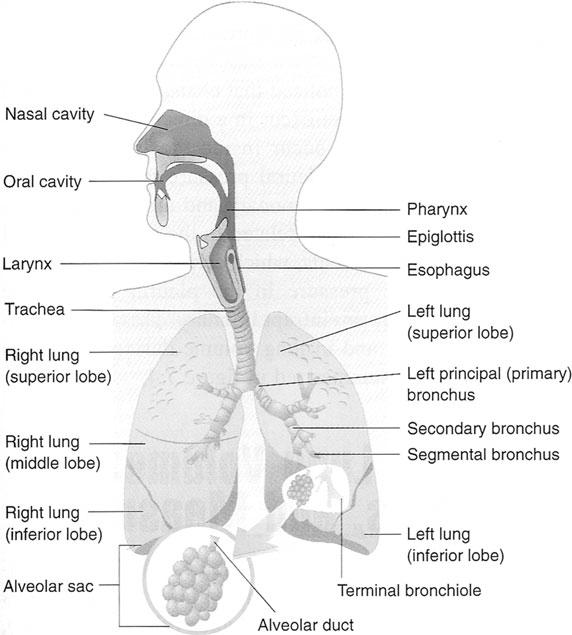
\includegraphics[width=0.55\textwidth]{91.png}
\caption{Diagrama de partes del sistema respiratorio. (Estos componentes también son importantes en la producción de la voz (Cap. 10). Las cuerdas vocales (o pliegues vocales) utilizadas al hablar se encuentran en la laringe). (De \cite{6}. Utilizado con permiso)}
\label{fig:9.1}
\end{figure}

\begin{figure}[htbp]
\centering
  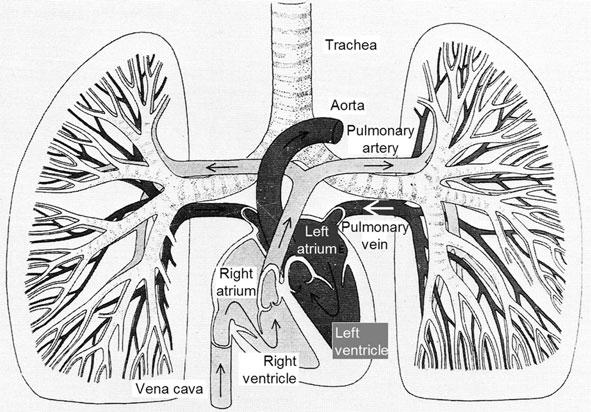
\includegraphics[width=0.7\textwidth]{92.png}
\caption{Se muestra la relación entre el pulmón y el corazón. Se muestran las primeras generaciones de la ramificación de los vasos de aire en los pulmones, las arterias pulmonares y las venas pulmonares. Estos tres sistemas pueden denominarse los tres «árboles» del pulmón. Tenga en cuenta que las arterias pulmonares están cerca de los bronquios, mientras que las venas pulmonares se encuentran solas (De \cite{9})}
\label{fig:9.2}
\end{figure}

\begin{SCfigure}[1.0][htbp]
\centering
  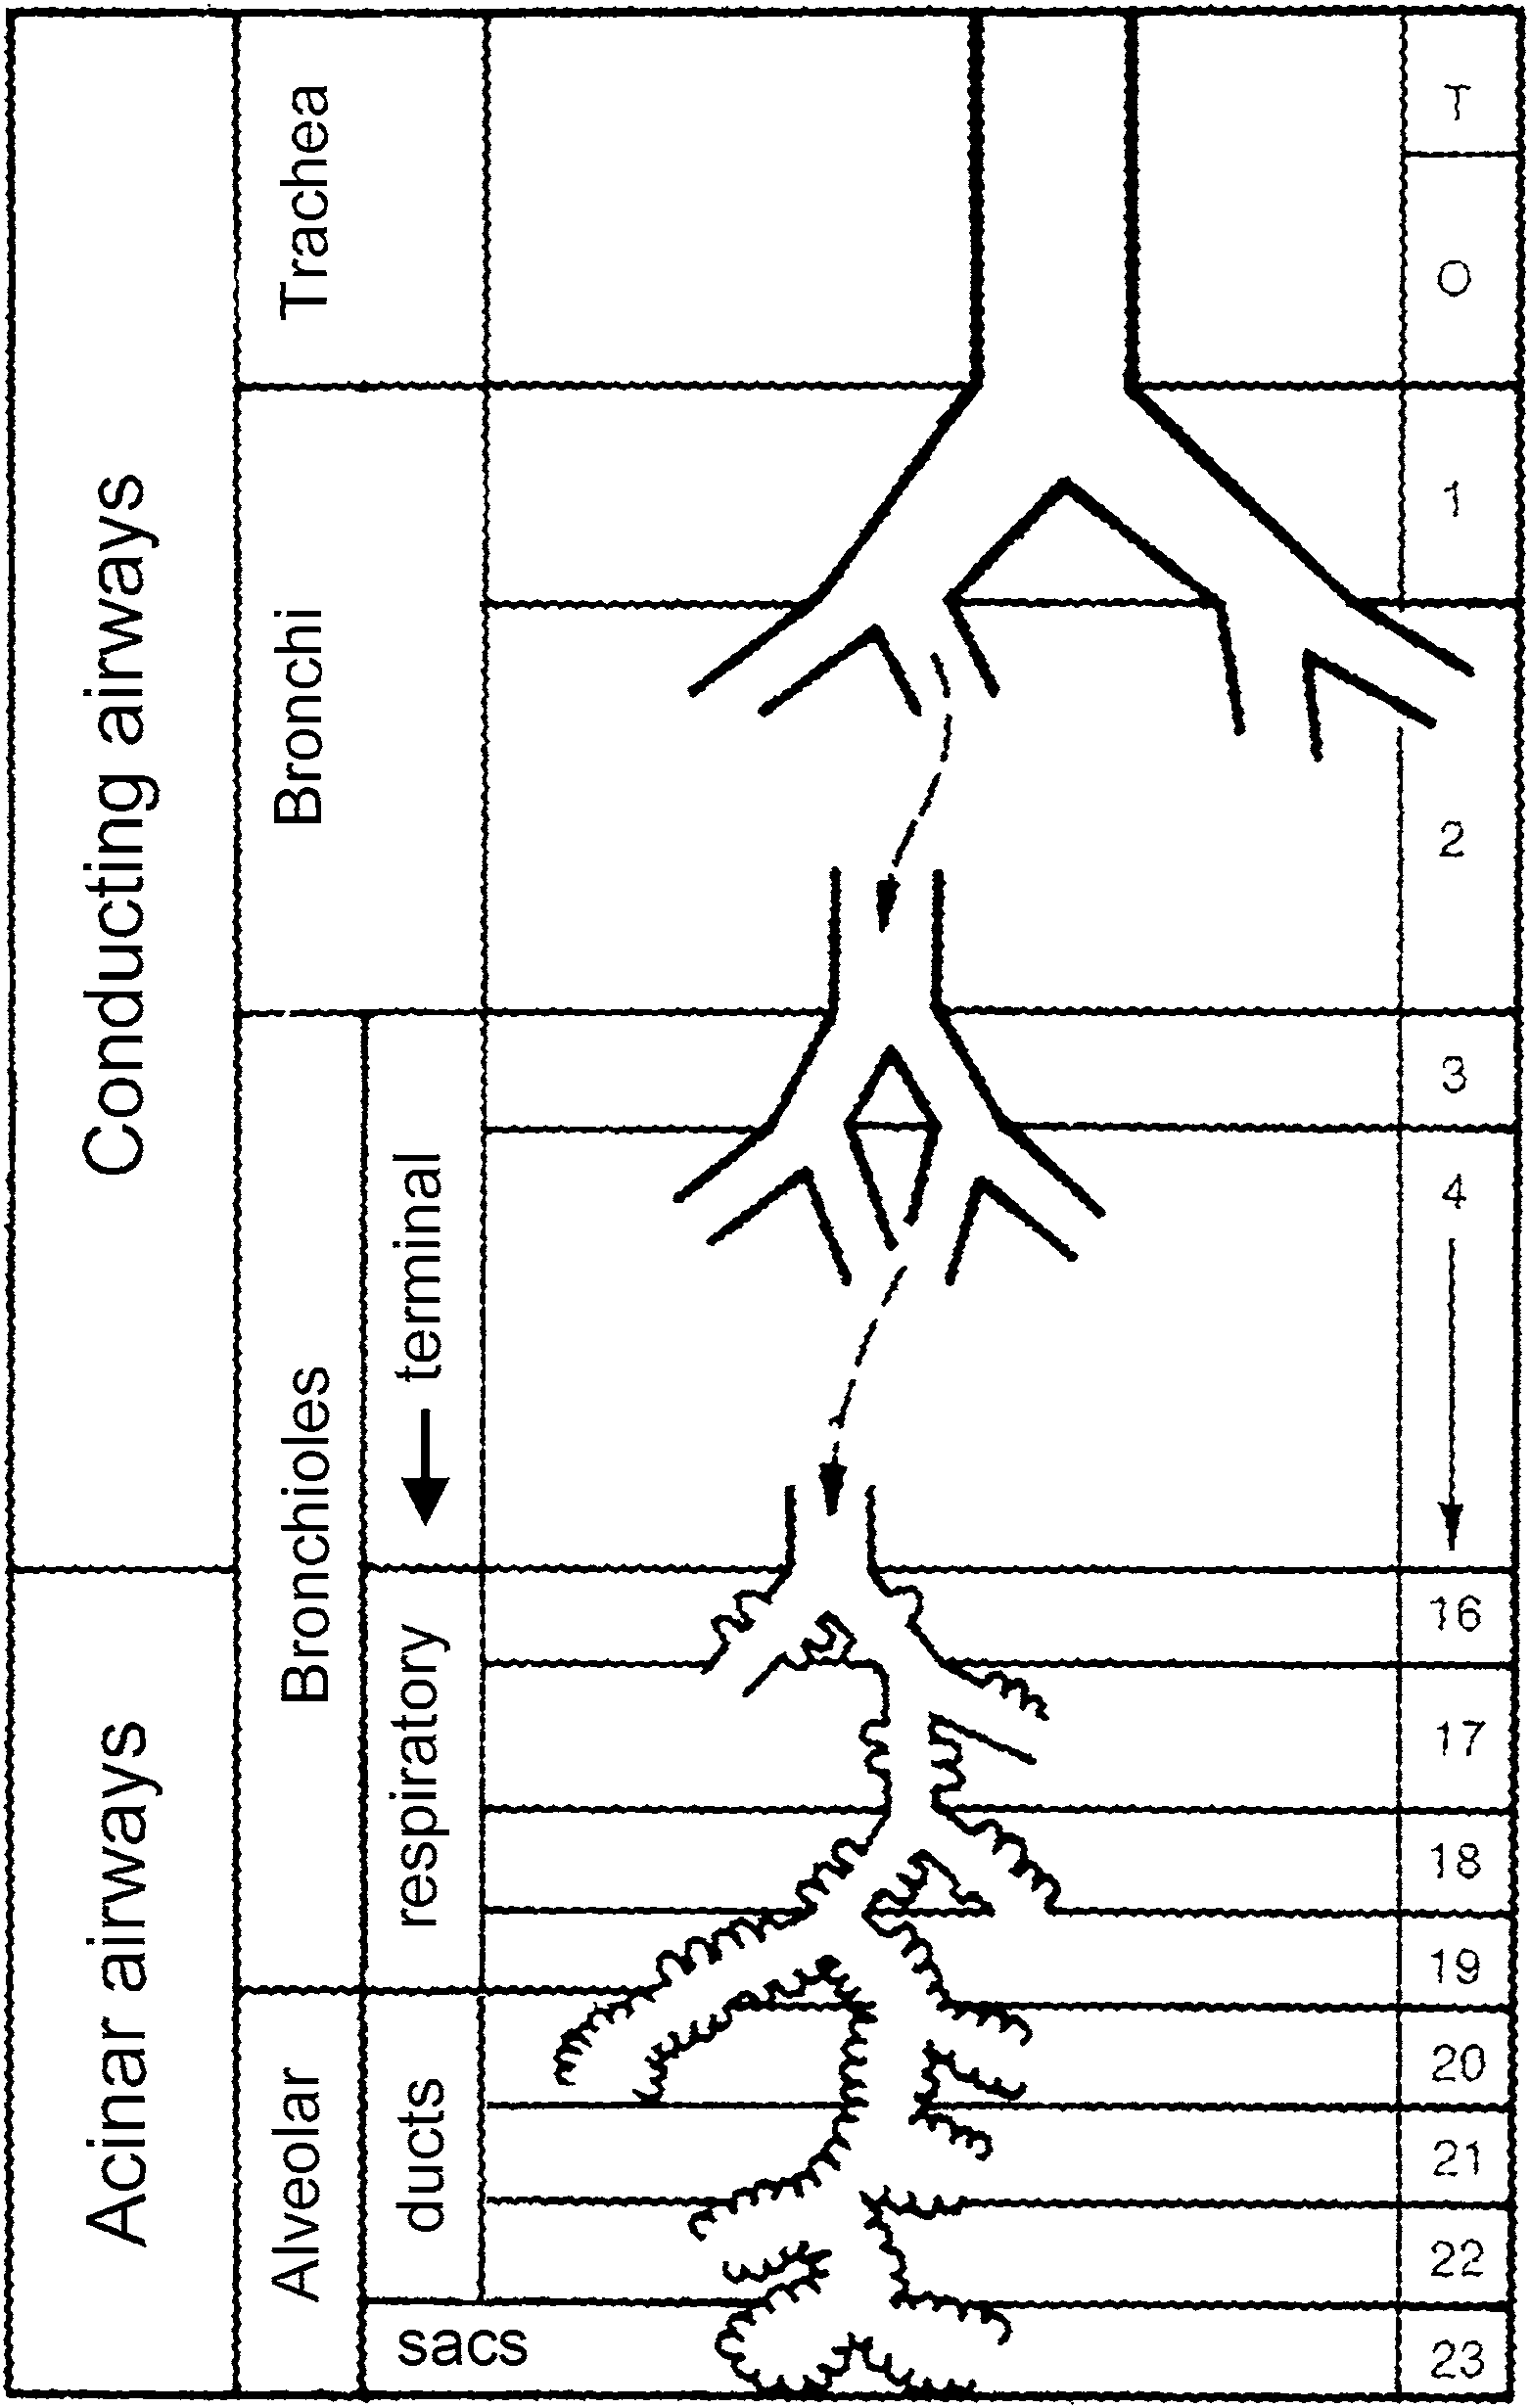
\includegraphics[width=0.45\textwidth]{93.png}
\caption{Bifurcaciones de las vías respiratorias pulmonares, que muestran el número de generación $z$ (De \cite{30})}
\label{fig:9.3}
\end{SCfigure}



El diámetro promedio de las vías respiratorias disminuye con la generación $z$, como $d(z) = 2^{-z/3}d(0)$ hasta la generación 16. Esta relación representa el diseño óptimo de un sistema ramificado de tubos en hidrodinámica. Hay alrededor de $3 \times 10^8$ alvéolos, cada uno de $\sim 0.2\text{}0.3\text{ mm}$ de diámetro, con paredes de $\sim 0.4\text{ }\mu\text{m}$ de espesor. Están en contacto con la sangre en los capilares pulmonares (Fig. 9.4), los cuales se forman a su vez tras subdividirse en 17 ramificaciones (Tabla 9.2, Figs. 9.2 y 9.5). El oxígeno se difunde desde los alvéolos hacia los glóbulos rojos, mientras que el dióxido de carbono se difunde desde la sangre hacia el aire en los alvéolos. El área superficial total de los alvéolos es de $\sim 80\text{ m}^2$ (en un rango de $50\text{}100\text{ m}^2$). El área de la superficie externa total de los pulmones es de solo $\sim 0.1\text{ m}^2$, por lo que la subdivisión en alvéolos resulta en un tremendo aumento del área superficial en contacto con la sangre, por un factor de casi 1,000. Este es también el factor por el cual aumenta la captación de oxígeno. Sin esto, nunca estaríamos ni cerca de satisfacer nuestras necesidades metabólicas de oxígeno. Nuestros pechos se expanden cuando respiramos porque el aire entrante que llena los alvéolos hace que cada uno de ellos sea más grande, tal como ocurre con las burbujas ordinarias. En \cite{13, 14, 28} se pueden encontrar modelos de la difusión de $\text{O}_2$ y $\text{CO}_2$ a través de las paredes de los alvéolos y de los capilares pulmonares y cómo progresa esta a lo largo de los capilares, junto con modelos sobre cómo se transportan estos gases entre los alvéolos y el resto de los pulmones (ventilación) y cómo los capilares suministran sangre a los tejidos (perfusión).

\begin{figure}[htbp]
\centering
  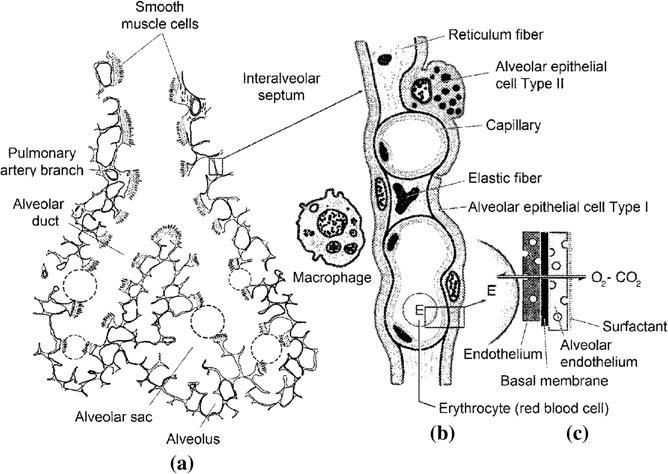
\includegraphics[width=0.7\textwidth]{94.png}
\caption{Los detalles de la bifurcación alveolar se muestran en (a). Estos alvéolos son sacos incrustados en lechos capilares. Los detalles de la interacción entre los alvéolos y los capilares se representan en (b) y (c) (De \cite{30})}
\label{fig:9.4}
\end{figure}





% Control de Calidad: 7 párrafos origen -> 7 párrafos salida. Mapeo 1:1 verificado. Sin omisiones.

\begin{table}[htbp]
\centering
\caption{Cuantificación aproximada del sistema bronquial}
\label{tab:9.1}
\small
\setlength{\tabcolsep}{4.5pt}
\begin{tabularx}{\textwidth}{>{\hsize=1.4\hsize}X >{\centering\arraybackslash\hsize=0.9\hsize}X >{\centering\arraybackslash\hsize=0.75\hsize}X >{\centering\arraybackslash\hsize=0.75\hsize}X >{\centering\arraybackslash\hsize=1.2\hsize}X >{\centering\arraybackslash\hsize=1.0\hsize}X >{\centering\arraybackslash\hsize=1.0\hsize}X}
\toprule
\textbf{Ramificación pulmonar} & \textbf{Generación $z$} & \textbf{Diámetro (mm)} & \textbf{Longitud (mm)} & \textbf{Área transversal total (cm$^2$)} & \textbf{Volumen (cm$^3$)} & \textbf{Velocidad del aire (cm/s)} \\
\midrule
Tráquea & 0 & 18.0 & 120.0 & 2.5 & 31 & 393 \\
Bronquio principal & 1 & 12.2 & 47.6 & 2.3 & 11 & 427 \\
Bronquio lobar & 2 & 8.3 & 19.0 & 2.1 & 4.0 & 462 \\
 & 3 & 5.6 & 7.6 & 2.0 & 1.5 & 507 \\
Bronquio segmental & 4 & 4.5 & 12.7 & 2.5 & 3.5 & 392 \\
 & 5 & 3.5 & 10.7 & 3.1 & 3.3 & 325 \\
Bronquios & 6 & 2.8 & 9.0 & 4.0 & 3.5 & 254 \\
con cartílago en la pared & 7 & 2.3 & 7.6 & 5.1 & 3.8 & 188 \\
 & 8 & 1.86 & 6.4 & 7.0 & 4.4 & 144 \\
 & 9 & 1.54 & 5.4 & 9.6 & 5.2 & 105 \\
 & 10 & 1.30 & 4.6 & 13 & 6.2 & 73.6 \\
Bronquio terminal & 11 & 1.09 & 3.9 & 20 & 7.6 & 52.3 \\
 & 12 & 0.95 & 3.3 & 29 & 9.8 & 34.4 \\
Bronquiolos & 13 & 0.82 & 2.7 & 44 & 12 & 23.1 \\
con músculo en la pared & 14 & 0.74 & 2.3 & 69 & 16 & 14.1 \\
 & 15 & 0.66 & 2.0 & 113 & 22 & 8.92 \\
Bronquiolo terminal & 16 & 0.60 & 1.65 & 180 & 30 & 5.40 \\
Bronquiolo respiratorio & 17 & 0.54 & 1.41 & 300 & 42 & 3.33 \\
Bronquiolo respiratorio & 18 & 0.50 & 1.17 & 534 & 61 & 1.94 \\
Bronquiolo respiratorio & 19 & 0.47 & 0.99 & 944 & 93 & 1.10 \\
Conducto alveolar & 20 & 0.45 & 0.83 & 1,600 & 139 & 0.60 \\
Conducto alveolar & 21 & 0.43 & 0.70 & 3,200 & 224 & 0.32 \\
Conducto alveolar & 22 & 0.41 & 0.59 & 5,900 & 350 & 0.18 \\
Saco alveolar & 23 & 0.41 & 0.50 & 12,000 & 591 & 0.09 \\
Alvéolos, 21 por conducto & -- & 0.28 & 0.23 & 3,200 & -- & -- \\
\bottomrule
\end{tabularx}
\begin{flushleft}
\small
Se asume que la velocidad del aire es de $1\text{ L/s}$. Los datos incluyen los de ambos pulmones. El número en cada generación es $2^z$ (para las generaciones $z = 0\text{}23$), y $300 \times 10^6$ para los alvéolos. Utilizando datos de \cite{8, 38}. Ver también \cite{39, 40}.
\end{flushleft}
\end{table}

El sistema circulatorio es el conducto para la transferencia de $\text{O}_2$ y $\text{CO}_2$ entre los alvéolos y los tejidos, por lo que debemos realizar un seguimiento de la presión parcial en cada sistema. Dentro de los alvéolos, la presión parcial de $\text{O}_2$ es $\simeq 105\text{ mmHg}$, que es menor que la de la atmósfera ($159\text{ mmHg} = 21\%$ de $760\text{ mmHg}$) debido al volumen muerto en el sistema respiratorio. La presión parcial de $\text{O}_2$ en la sangre de los capilares pulmonares aumenta de 40 a $\simeq 100\text{ mmHg}$ después de que el $\text{O}_2$ se transfiere desde los alvéolos, y esta es la presión parcial en las venas pulmonares y las arterias sistémicas. La presión parcial de $\text{O}_2$ en los tejidos es de $40\text{ mmHg}$, de modo que tras la transferencia de $\text{O}_2$ desde los capilares a los tejidos circundantes, la presión parcial en las venas sistémicas y las arterias pulmonares también es de $\simeq 40\text{ mmHg}$, y luego se incrementa nuevamente a $100\text{ mmHg}$ en los pulmones.

De manera similar, dentro de los alvéolos la presión parcial de $\text{CO}_2$ es $\simeq 40\text{ mmHg}$; esta es mucho mayor que la de la atmósfera ($\sim 0.3\text{ mmHg}$), nuevamente debido al volumen muerto. La presión parcial de $\text{CO}_2$ en la sangre en los capilares pulmonares disminuye de 46 a $\simeq 40\text{ mmHg}$ después de que el $\text{CO}_2$ se transfiere a los alvéolos, y esta es la presión parcial en las venas pulmonares y las arterias sistémicas. La presión parcial de $\text{CO}_2$ en los tejidos es de $46\text{ mmHg}$, de modo que después de la transferencia de $\text{CO}_2$ a los capilares desde los tejidos, la presión parcial en las venas sistémicas y las arterias pulmonares es también de $\simeq 46\text{ mmHg}$, y luego disminuye nuevamente a $40\text{ mmHg}$ en los pulmones. Con el avance de la edad, la diferencia entre los niveles de $\text{O}_2$ arterial y venoso disminuye, lo que indica que el cuerpo está utilizando menos oxígeno. En el ejercicio máximo en hombres entrenados en resistencia, esta diferencia disminuye en un $\sim 8\%$ desde $\sim 16.7\text{ mL}(\text{O}_2)/100\text{ mL}(\text{sangre})$ a los 28 años de edad hasta $\sim 15.2\text{ mL}/100\text{ mL}$ a los 60 años de edad \cite{36}.

\section{La física de los alvéolos}

Los alvéolos son similares a burbujas interconectadas. Dentro de ellos la presión es $P_{\text{in}}$ y fuera la presión es $P_{\text{out}}$, con $\Delta P = P_{\text{in}} - P_{\text{out}}$, y tienen un radio $R$. La ley de Laplace para una esfera (7.9) es
\begin{equation}
\Delta P = \frac{2T}{R},
\label{eq:9.1}
\end{equation}
donde $T$ es la tensión en las paredes de la esfera. La fuente principal de esta tensión en los alvéolos no se encuentra dentro de las paredes, sino en las superficies. Esta contribución se denomina tensión superficial $\gamma$, la cual tiene las mismas unidades que $T$ (de fuerza/longitud o energía/área). En burbujas típicas, como las burbujas de jabón, ambas superficies contribuyen con la misma tensión superficial, por lo que $T$ se reemplaza por $2\gamma$. Por lo tanto, encontramos
\begin{equation}
\Delta P = P_{\text{in}} - P_{\text{out}} = \frac{4\gamma}{R}.
\label{eq:9.2}
\end{equation}
Para la interfaz agua/aire, $\gamma \simeq 7.2 \times 10^{-4}\text{ N/m}$ (Tabla 7.2). En los alvéolos, sin embargo, solo la tensión superficial de la superficie interna es realmente importante porque es una interfaz fluido/aire y tiene una tensión superficial mayor que la interfaz fluido/fluido de la superficie externa, por lo que
\begin{equation}
\Delta P_{\text{alveoli}} = P_{\text{in}} - P_{\text{out}} = \frac{2\gamma}{R}.
\label{eq:9.3}
\end{equation}

% Control de Calidad: 3 párrafos origen -> 3 párrafos salida. Mapeo 1:1 verificado. Sin omisiones.

\begin{table}[htbp]
\centering
\caption{Estructura de ramificación de la red arterial pulmonar}
\label{tab:9.2}
\small
\begin{tabularx}{\textwidth}{>{\hsize=1.4\hsize}X >{\centering\arraybackslash\hsize=1.2\hsize}X >{\centering\arraybackslash\hsize=0.7\hsize}X >{\centering\arraybackslash\hsize=0.7\hsize}X}
\toprule
\textbf{Orden de ramificación pulmonar} & \textbf{Número de ramificaciones de cada orden} & \textbf{Longitud del vaso (mm)} & \textbf{Diámetro del vaso (mm)} \\
\midrule
1 & 1 & 90.5 & 30.0 \\
2 & 3 & 32.0 & 14.83 \\
3 & 8 & 10.9 & 8.06 \\
4 & 20 & 20.7 & 5.82 \\
5 & 66 & 17.9 & 3.65 \\
6 & 203 & 10.5 & 2.09 \\
7 & 675 & 6.6 & 1.33 \\
8 & 2,290 & 4.69 & 0.85 \\
9 & 5,861 & 3.16 & 0.525 \\
10 & 17,560 & 2.10 & 0.351 \\
11 & 52,550 & 1.38 & 0.224 \\
12 & 157,400 & 0.91 & 0.138 \\
13 & 471,300 & 0.65 & 0.086 \\
14 & 1,411,000 & 0.44 & 0.054 \\
15 & 4,226,000 & 0.29 & 0.034 \\
16 & 12,660,000 & 0.20 & 0.021 \\
17 & 300,000,000 & 0.13 & 0.013 \\
\bottomrule
\end{tabularx}
\begin{flushleft}
\small
Utilizando datos de \cite{8, 33}.
\end{flushleft}
\end{table}

\begin{figure}[htbp]
\centering
  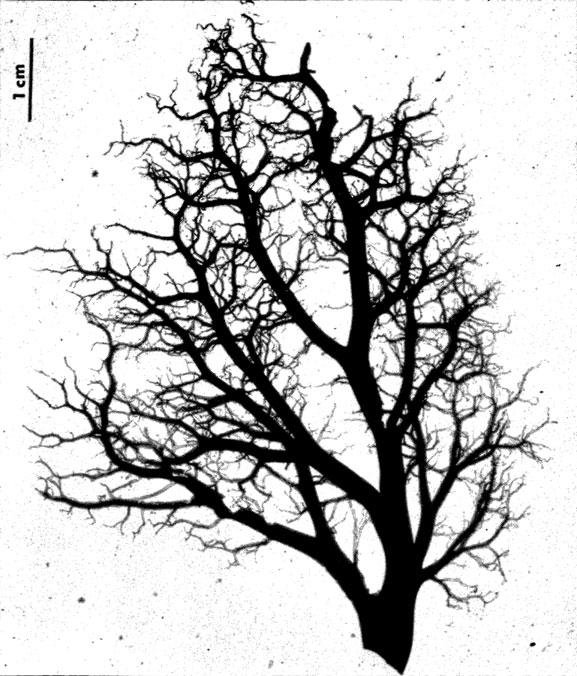
\includegraphics[width=0.55\textwidth]{95.png}
\caption{Un molde de elastómero de silicona del árbol venoso del pulmón de un gato. La presión venosa fue de $-7\text{ cmH}_2\text{O}$ ($= -5\text{ mmHg}$), la presión de las vías respiratorias fue de $10\text{ cmH}_2\text{O}$ ($= 7\text{ mmHg}$), y la presión pleural fue de $0\text{ cmH}_2\text{O}$ (De \cite{9})}
\label{fig:9.5}
\end{figure}


Existe una inestabilidad aparente que aparentemente conduce a una situación irrazonable en burbujas o alvéolos interconectados. Considere dos burbujas que inicialmente no están interconectadas, como en la Fig. 9.6, debido a que hay un tapón entre ellas. La burbuja \#1 tiene una presión interna $P_1$ y un radio $R_1$, y la burbuja \#2 tiene una presión interna $P_2$ y un radio $R_2$. (Debido a que la diferencia entre la presión interior y exterior de la burbuja es lo significativo, la presión externa es igual a cero). En equilibrio, la presión interna $P_{\text{internal}} = 4\gamma/R$ para cada burbuja. (Que este factor sea 4 o 2 no es significativo aquí). Digamos que la burbuja \#2 es la burbuja más pequeña. Debido a que $R_2 < R_1$, en equilibrio $P_2 > P_1$; la burbuja más pequeña tiene la presión interna más alta. Si se abre el tapón, el aire fluirá desde la presión más alta hacia la presión más baja y, por lo tanto, desde la burbuja más pequeña hacia la burbuja más grande. La pérdida de aire en la burbuja \#2 la hace más pequeña. Con este radio más pequeño, la presión interna de equilibrio aumenta. Debido a que esta presión sigue siendo mayor que en la burbuja \#1, el aire continúa fluyendo desde la burbuja más pequeña hacia la burbuja más grande, hasta que colapsa.

\begin{SCfigure}[0.75][htbp]
\centering
  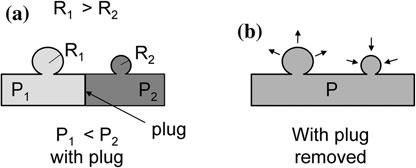
\includegraphics[width=0.6\textwidth]{96.png}
\caption{Inestabilidad de las burbujas, según la ley de Laplace. Esto asume que la tensión superficial no cambia con el radio de la burbuja (o alvéolo). La presión externa es 0}
\label{fig:9.6}
\end{SCfigure}



Esto implica que el más grande de los cientos de millones de alvéolos se haría cada vez más grande a expensas de todos los más pequeños, y el sistema de alvéolos que hemos descrito para los pulmones no podría ser estable. ¿Qué hay de malo en este escenario? No hay ningún error en nuestro razonamiento; sin embargo, hemos hecho una suposición que no es precisa para los alvéolos. Asumimos implícitamente que la tensión superficial no es una función del radio $R$. Existe un surfactante en las superficies de los alvéolos de personas sanas, que contiene dipalmitoil fosfatidilcolina o DPPC, que hace que $\gamma(R)$ sea independiente de $R$ desde 0 hasta un tamaño crítico ($R_0$). Con $\Delta P = 2\gamma(R)/R$, algunas burbujas se vuelven más grandes y otras más pequeñas como en la Fig. 9.6. Sin embargo, eventualmente $\gamma(R)$ aumenta con un $R$ mayor más rápido de lo que lo hace el propio $R$, por lo que $\Delta P$ comienza a aumentar con un $R$ aún mayor. Tal sistema de alvéolos interconectados es estable.

Podemos ver cómo puede ocurrir tal dependencia de $\gamma(R)$ con el siguiente modelo. La superficie de un alvéolo puede estar cubierta ya sea con una lipoproteína o por agua; la tensión superficial de la lipoproteína es mucho menor ($\gamma_{\text{lung}} = 1 \times 10^{-3}\text{ N/m}$) que la del agua ($\gamma_{\text{water}} = 7.2 \times 10^{-2}\text{ N/m}$ ($= 72\text{ dinas/cm}$)). Suponiendo que el alvéolo es esférico, para un radio particular $R_0$ hay exactamente una monocapa de lipoproteína en toda la superficie y en ese radio la tensión superficial es $\gamma_{\text{lung}}$ sobre el área superficial $4 \pi R_0^2$. Si este alvéolo se vuelve más pequeño, de modo que $R < R_0$, tiene varias monocapas de lipoproteína en su superficie y su tensión superficial sigue siendo $\gamma_{\text{lung}}$, por lo que
\begin{equation}
\gamma(R) = \gamma_{\text{lung}} \quad \text{para } R \le R_0.
\label{eq:9.4}
\end{equation}

Si este mismo alvéolo en cambio se vuelve más grande, de modo que $R > R_0$, tiene una monocapa de lipoproteína sobre solo una porción de su superficie (de área superficial $4\pi R_0^2$ debido a que la capa no puede volverse más pequeña que una monocapa) y agua sobre el resto de la superficie (de área $4\pi R^2 - 4\pi R_0^2$). Por lo tanto, la tensión superficial promedio es
\begin{equation}
\gamma(R) = \frac{4\pi R_0^2 \gamma_{\text{lung}} + (4\pi R^2 - 4\pi R_0^2)\gamma_{\text{water}}}{4\pi R^2} \quad \text{para } R > R_0
\label{eq:9.5}
\end{equation}
o
\begin{equation}
\gamma(R) = \gamma_{\text{water}} - \frac{R_0^2}{R^2} (\gamma_{\text{water}} - \gamma_{\text{lung}}) \quad \text{para } R > R_0.
\label{eq:9.6}
\end{equation}
Esto se aproxima a la $\gamma_{\text{water}}$ mucho mayor para $R \gg R_0$ a una tasa que es más rápida que $R$, por lo que los alvéolos serán estables.

% Control de Calidad: 4 párrafos origen -> 4 párrafos salida. Mapeo 1:1 verificado. Sin omisiones.

Debido a que esta lipoproteína está solo en una de las superficies, la condición de estabilidad es $\Delta P = 2\gamma/R$. Para $R > R_0$, hay un equilibrio estable cuando $d(\Delta P)/dR = d[2\gamma_{\text{water}}/R - 2(R_0^2/R^3)(\gamma_{\text{water}} - \gamma_{\text{lung}})]/dR = 0$ o
\begin{equation}
\frac{d(\Delta P)}{dR} = -\frac{2\gamma_{\text{water}}}{R^2} + \frac{6 R_0^2}{R^4} (\gamma_{\text{water}} - \gamma_{\text{lung}}) = 0
\label{eq:9.7}
\end{equation}
o
\begin{equation}
R_{\text{eq}} = \sqrt{\frac{3\gamma_{\text{water}} - \gamma_{\text{lung}}}{\gamma_{\text{water}}}} R_0.
\label{eq:9.8}
\end{equation}
Debido a que $\gamma_{\text{water}} \gg \gamma_{\text{lung}}$, el radio de equilibrio es $R_{\text{eq}} \simeq \sqrt{3}R_0$.

La Figura 9.7 muestra que esta tensión superficial del surfactante en el pulmón disminuye desde $5 \times 10^{-2}\text{ N/m}$ ($50\text{ dinas/cm}$) hasta cero a medida que el área de la película se hace más pequeña. Los alvéolos son típicamente estables a aproximadamente 1/4 de su tamaño máximo.

\begin{figure}[htbp]
\centering
  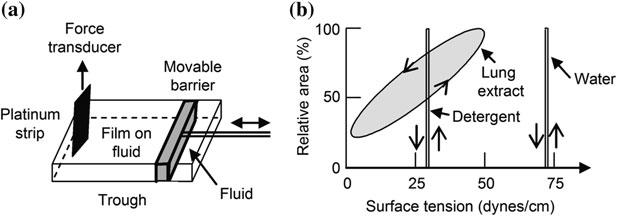
\includegraphics[width=0.65\textwidth]{97.png}
\caption{Tensión superficial en las paredes alveolares (extracto pulmonar) en (b), según lo medido por la balanza superficial en (a) que mide la tensión superficial frente al área. También se muestran mediciones similares para detergente y agua (Basado en \cite{12, 42})}
\label{fig:9.7}
\end{figure}



Una función del surfactante es proporcionar estabilidad al alvéolo. Otra función es disminuir la cantidad de fuerza que debe suministrar el diafragma para inflar los alvéolos. Con $\gamma_{\text{water}} = 7.2 \times 10^{-2}\text{ N/m}$ y $R = 0.05\text{ mm}$ de los alvéolos cuando están colapsados (y necesitan ser inflados), la ecuación (9.3) da $\Delta P_{\text{alveoli}} = 2.9 \times 10^3\text{ N/m}^2 = 22\text{ mmHg}$. El área del músculo del diafragma de un adulto es de aproximadamente $500\text{ cm}^2$, por lo que la fuerza que necesita ejercer para expandir los alvéolos para la respiración es de $\sim 150\text{ N}$ lo que corresponde a un peso con una masa de $15\text{ kg}$. Con la tensión superficial más baja del surfactante pulmonar, esta fuerza es más de un orden de magnitud menor y la respiración es más fácil, especialmente para los lactantes. Esto explica por qué las personas con surfactante insuficiente con enfermedad de membrana hialina tienen dificultad para respirar.

\FloatBarrier
\section{Física de la respiración}

Cada pulmón está rodeado por una membrana de saco dentro de la cavidad torácica. Podemos imaginar el saco pleural como un globo, como en la Fig. 9.8, lleno de líquido intrapleural. La pared interna de este saco, la pleura visceral (membrana), se adhiere a la pared externa del pulmón. La pared externa de este saco, la pleura parietal (membrana), se adhiere a la pared torácica. Es la elasticidad del pulmón lo que separa las dos membranas pleurales, y esto causa una ligera disminución de la presión del saco pleural en relación con la presión atmosférica, de $-4\text{ mmHg}$ a $-6\text{ mmHg}$. Esta diferencia de presión es lo que mantiene los pulmones expandidos y evita que colapsen. La «fuerza impulsora» mecánica para controlar el volumen pulmonar es la presión transpulmonar, que es la diferencia entre la presión en los alvéolos de los pulmones y aquella alrededor del pulmón en el saco pleural, la cual se denomina presión intrapleural (o pleural). (Las presiones alveolar y pleural son presiones manométricas, referenciadas a la presión atmosférica).

\begin{figure}[htbp]
\centering
  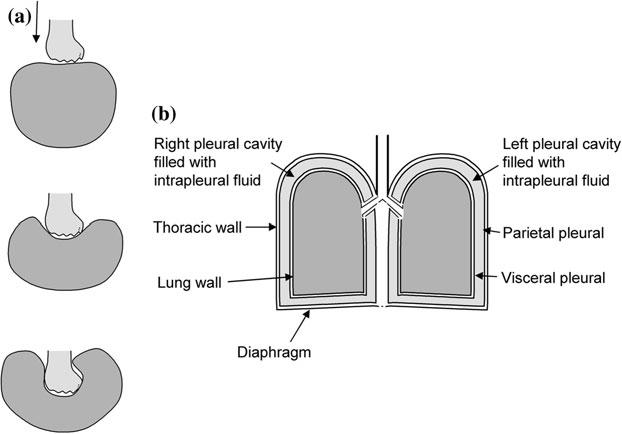
\includegraphics[width=0.7\textwidth]{98.png}
\caption{a Empujar un puño en un globo es análogo a los pulmones en la cavidad pleural. b Esquema de los pulmones en las cavidades pleurales (Basado en \cite{34})}
\label{fig:9.8}
\end{figure}



Los pulmones se expanden y se contraen por el movimiento de las estructuras que los rodean a través de los músculos inspiratorios y espiratorios. Esto ocurre de dos maneras (Fig. 9.9), de las cuales solo la primera se utiliza durante la respiración tranquila. (1) El diafragma se mueve hacia abajo para alargar la cavidad torácica (tirando de la parte inferior de los pulmones hacia abajo) durante la inspiración. Durante la respiración tranquila, los pulmones se contraen por el retroceso elástico natural de los pulmones y de la pared torácica, con el diafragma relajado, mientras que en la respiración más pesada esta contracción se acelera por la contracción de los músculos abdominales que empujan el contenido abdominal y luego el diafragma hacia arriba para acortar la cavidad torácica. (2) Las costillas son elevadas por los músculos del cuello para aumentar el diámetro anteroposterior (de adelante hacia atrás) de la cavidad torácica y son deprimidas (descendidas) por los rectos abdominales para disminuirlo. Esto causa la expansión y contracción de la cavidad torácica, respectivamente, debido a que las costillas se inclinan hacia afuera y tienen áreas de sección transversal transversales más grandes en las secciones inferiores; esto puede aumentar el espesor anteroposterior del tórax en aproximadamente un 20\% durante la inspiración.

\begin{figure}[htbp]
  \centering
  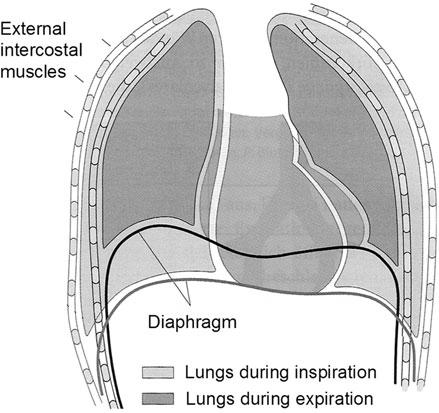
\includegraphics[width=0.55\textwidth]{99.png}
  \caption{Expansión y contracción de la caja torácica durante la espiración y la inspiración, mostrando las costillas, los pulmones y el corazón, los músculos intercostales externos (que se contraen durante la inspiración para elevar la caja torácica y ensancharla lateralmente de modo que la caja aumente en las tres dimensiones) y el diafragma (que se contrae para aumentar la dimensión vertical de la caja durante la inspiración) (De \cite{31}).}
  \label{fig:9.9}
\end{figure}



¿Cómo ayuda esto a introducir aire en los pulmones? Antes de la inspiración, hay presión atmosférica en los pulmones. La fuerza de atracción de la pleura visceral hacia la pleura parietal y la fuerza hacia afuera de la pared pulmonar externa debido a la presión menor que la atmosférica en el saco pleural ($\sim -4\text{ mmHg}$) hacen que cada pulmón se expanda. En equilibrio, su suma está equilibrada por la tendencia de los pulmones a contraerse debido a su elasticidad. Este equilibrio de fuerzas previo a la inspiración se muestra en la Fig. 9.10. Ya no están en equilibrio durante la inspiración.

\begin{figure}[htbp]
  \centering
  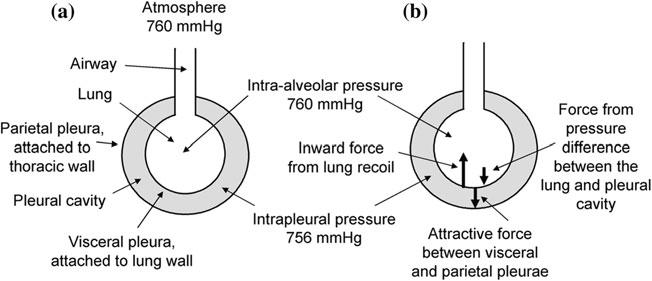
\includegraphics[width=0.8\textwidth]{910.png}
  \caption{Balance de fuerzas de la pleura visceral/pared externa del pulmón durante la preinspiración. Tenga en cuenta que las fuerzas son realmente normales a la pared en todas partes, no solo en la parte inferior como se representa (Basado en \cite{34}).}
  \label{fig:9.10}
\end{figure}



Los pasos de la inspiración (inhalación) se muestran en la Fig. 9.11. Los músculos inspiratorios (diafragma e intercostales externos) aumentan las dimensiones de la caja torácica (la

\begin{figure}[htbp]
  \centering
  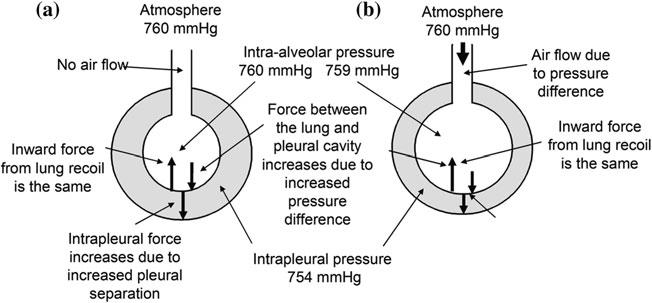
\includegraphics[width=0.8\textwidth]{911.png}
  \caption{a El desequilibrio de fuerzas al inicio de la contracción muscular inspiratoria (y la expansión de la pared torácica/pleura parietal) conduce a una (b) presión subatmosférica en los pulmones y al flujo de aire hacia los pulmones durante la inspiración. (Compare esto con el balance de fuerzas preinspiratorio de la Fig. 9.10) (Basado en \cite{34}).}
  \label{fig:9.11}
\end{figure}



% Control de Calidad: 7 párrafos origen -> 7 párrafos salida. Mapeo 1:1 verificado. Sin omisiones.

cavidad torácica). Esto causa que la pleura visceral y la parietal se separen. El volumen pulmonar aumenta entonces porque (1) la atracción de la pleura visceral y la parietal aumenta a medida que se separan más y (2) esta separación causa que $P_{\text{lung}} - P_{\text{pleura}}$ disminuya aún más, de $\sim -4$ a $\sim -6\text{ mmHg}$ (es decir, de $\sim 756$ a $754\text{ mmHg}$ de presión absoluta). Debido a que ambas fuerzas en la dirección de la expansión pulmonar aumentan, ahora vencen la elasticidad de los pulmones que favorece la contracción pulmonar, y el pulmón se expande. La presión en los pulmones y los alvéolos disminuye de $\sim 0$ a $\sim -1\text{ mmHg}$ (es decir, de $\sim 760$ a $759\text{ mmHg}$ de presión absoluta), y luego el aire fluye desde la boca y la nariz hacia los pulmones. Durante la respiración normal, la espiración es automática y no requiere contracción muscular. La contracción muscular es necesaria durante el ejercicio intenso para inhalar más aire fresco y espirar activamente el aire viciado.

\FloatBarrier
\section{Volumen de los Pulmones} \label{sec:9.4}

El volumen de los pulmones depende de la presión transpulmonar, como se observa en la Fig. 9.12 para un pulmón extirpado. Las curvas de inflado y desinflado no son iguales; al igual que en la discusión sobre viscoelasticidad del Cap. 4, esta asimetría se denomina histéresis.

\begin{figure}[htbp]
  \centering
  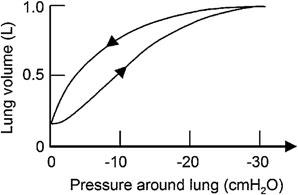
\includegraphics[width=0.7\textwidth]{912.png}
  \caption{Medición de la curva presión-volumen de un pulmón extirpado, que muestra histéresis en el inflado y desinflado (Basado en \cite{42}).}
  \label{fig:9.12}
\end{figure}



El volumen de los pulmones durante las diferentes etapas de la respiración normal y profunda es un buen diagnóstico de la funcionalidad pulmonar. Se mide fácilmente utilizando un espirómetro (Fig. 9.13). La Figura 9.13 muestra una de estas mediciones durante diferentes tipos de respiración. En este ejemplo, durante la respiración normal se observa que el volumen pulmonar oscila entre $3.2\text{ L}$ después de una inspiración normal y $2.2\text{ L}$ después de una espiración normal. La diferencia es el volumen corriente ($V_T$) ($\sim 1\text{ L}$), que es el volumen pulmonar habitual utilizado durante la respiración en reposo. El volumen después de una espiración normal es la capacidad residual funcional (CRF). Después de una inspiración profunda, el volumen pulmonar es la capacidad pulmonar total (CPT), $\sim 6\text{ L}$. Esto supera el volumen después de una inspiración normal por el volumen de reserva inspiratoria (VRI, que también es uno de los apodos del autor). Después de una espiración profunda, el volumen restante es el volumen residual (VR), $\sim 1\text{ L}$. La diferencia en los volúmenes pulmonares después de una inspiración profunda y una espiración profunda es la capacidad vital (CV) $\sim 5\text{ L}$, que también es igual a la capacidad pulmonar total menos el volumen residual. Después de una espiración profunda, el volumen pulmonar es menor que el posterior a una espiración normal por el volumen de reserva espiratoria (VRE), que también equivale a la capacidad residual funcional menos el volumen residual.

\begin{figure}[htbp]
  \centering
  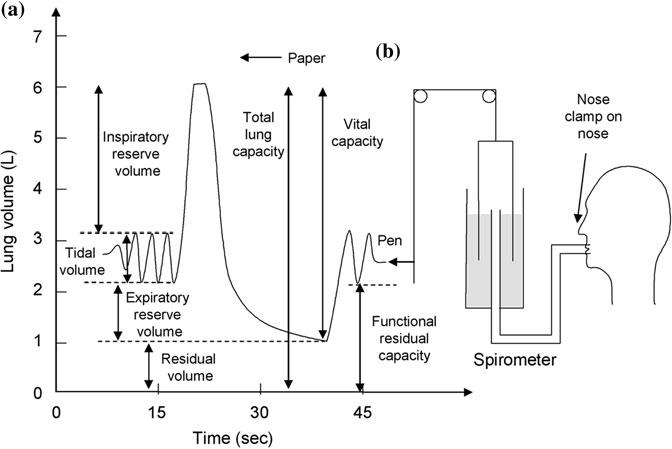
\includegraphics[width=0.7\textwidth]{913.png}
  \caption{a Cambios en el volumen pulmonar durante los ciclos respiratorios, b junto con un esquema de un espirómetro (Basado en \cite{3, 42}).}
  \label{fig:9.13}
\end{figure}



Durante el embarazo, la tasa de inhalación aumenta en un $\sim 30$--$50\%$, debido al aumento del volumen corriente ($V_T$) y de la frecuencia respiratoria \cite{19}. El consumo de oxígeno aumenta en un $\sim 20$--$40\%$ para satisfacer las necesidades del feto y la placenta, así como las necesidades adicionales de los órganos de la madre.

La capacidad vital es una medida importante de qué tan bien están funcionando los pulmones. (Más importante aún, se necesita una capacidad vital robusta para poder inflar globos). La capacidad residual funcional es el volumen de aire viciado que normalmente se mezcla con el aire nuevo (el volumen corriente ($V_T$)). También existe el espacio muerto. Parte es anatómico ($0.15\text{ L}$), debido a la tráquea y los bronquios, y parte es espacio muerto alveolar fisiológico, donde los alvéolos no tienen acceso a la sangre. Con la edad avanzada, la capacidad pulmonar total no cambia, pero la capacidad vital disminuye. El espacio muerto alveolar aumenta, lo que afecta el nivel de oxígeno en las arterias, pero no la eliminación de dióxido de carbono \cite{32, 37}.

% Control de Calidad: 5 párrafos origen -> 5 párrafos salida. Mapeo 1:1 verificado. Sin omisiones.

Sabemos que inhalamos aire que es $\sim 80\%\text{ N}_2 / 20\%\text{ O}_2 / 0\%\text{ CO}_2$, ignorando nuevamente el vapor de agua y el $\text{Ar}$, el cual se mezcla con el aire viciado, y después de la difusión a través de las paredes de los alvéolos espiramos aire que es $\sim 80\%\text{ N}_2 / 16\%\text{ O}_2 / 4\%\text{ CO}_2$. ¿Cuál es la composición de este aire viciado? Llamemos a su composición $80\%\text{ N}_2 / x\%\text{ O}_2 / y\%\text{ CO}_2$. Después de la inspiración, los pulmones tienen un volumen corriente ($V_T$) de aire al $80\%\text{ N}_2 / 20\%\text{ O}_2 / 0\%\text{ CO}_2$ que se ha mezclado con una capacidad residual funcional de aire al $80\%\text{ N}_2 / x\%\text{ O}_2 / y\%\text{ CO}_2$. Si el volumen corriente ($V_T$) es una fracción $\alpha$ de este volumen, la fracción de volumen de la capacidad residual funcional es $1 - \alpha$. Después de la inhalación, la composición del aire en los pulmones es $80\%\text{ N}_2 / [20\alpha + (1 - \alpha)x]\%\text{ O}_2 / (1 - \alpha)y\%\text{ CO}_2$. Supongamos que una fracción $\beta$ de todo el aire inhalado es absorbida por los pulmones. Esto significa que se absorbe una fracción $\beta$ del $20\alpha\%\text{ O}_2$ en los pulmones, lo cual es $20\alpha\beta\%\text{ O}_2$. Hay un aumento igual de $20\alpha\beta\%$ en el $\text{CO}_2$ que difunde hacia los pulmones. Así, después de la transferencia de oxígeno y dióxido de carbono, el aire en los pulmones tiene una composición de $80\%\text{ N}_2 / [20\alpha - 20\alpha\beta + (1 - \alpha)x]\%\text{ O}_2 / [20\alpha\beta + (1 - \alpha)y]\%\text{ CO}_2$, el cual es espirado. Por lo tanto, las fracciones de oxígeno y dióxido de carbono son, respectivamente,
\begin{equation}
16\% = [20\alpha - 20\alpha\beta + (1 - \alpha)x]\% \label{eq:9.9}
\end{equation}
\begin{equation}
4\% = [20\alpha\beta + (1 - \alpha)y]\% \label{eq:9.10}
\end{equation}

La fracción del volumen corriente ($V_T$) es $\alpha = 1/3$ y la fracción de oxígeno inhalado que es absorbido por los pulmones es $\beta = 1/4$. Esto da $x = 16.5$ e $y = 3.5$, por lo que el aire viciado en los pulmones tiene una composición de $80\%\text{ N}_2 / 16.5\%\text{ O}_2 / 3.5\%\text{ CO}_2$. (Este aire está claramente lo suficientemente oxigenado como para ser útil durante la reanimación boca a boca).

\FloatBarrier
\section{Respiración en Condiciones Habituales e Inusuales} \label{sec:9.5}

\subsection{Flujo de Aire Durante la Respiración} \label{subsec:9.5.1}

Durante la inspiración, el aire fluye porque la presión es menor en los pulmones y alvéolos en una cantidad positiva $\Delta P$ que en la atmósfera. La cantidad de aire que fluye está determinada por la resistencia y la compliancia del sistema respiratorio.

La compliancia del pulmón es de $\sim 0.2\text{ L/cmH}_2\text{O}$ y disminuye para una persona normal con presiones de expansión más altas, como se observa por la pendiente decreciente en la Fig. 9.12. Al intentar evaluar el rendimiento pulmonar, la compliancia específica del pulmón es quizás más significativa, para la cual la compliancia pulmonar se normaliza mediante una característica del tamaño de la persona, como un volumen pulmonar característico (CRF, CV, CPT, etc.), el peso seco del pulmón o el peso corporal. La elasticidad del tórax, así como la del pulmón, contribuye a la compliancia pulmonar.

La resistencia de las vías respiratorias es dominante dentro de las generaciones de bronquios de tamaño intermedio, como se ve en la Fig. 9.14a y en el Problema 9.21. La ley de Poiseuille (7.24) se puede utilizar para calcular la resistencia de las vías respiratorias en los pulmones (Problemas 9.21--9.23) y otros conductos (Problemas 9.16 y 9.18). La resistencia total de las vías respiratorias es típicamente de $\sim 2\text{ cmH}_2\text{O}/(\text{L/s})$ durante la respiración normal y disminuye con el aumento del tamaño pulmonar (Fig. 9.14b). La resistencia respiratoria aumenta durante el embarazo \cite{19}. (Se mide como en la Fig. 9.17 a continuación).

\begin{figure}[htbp]
  \centering
  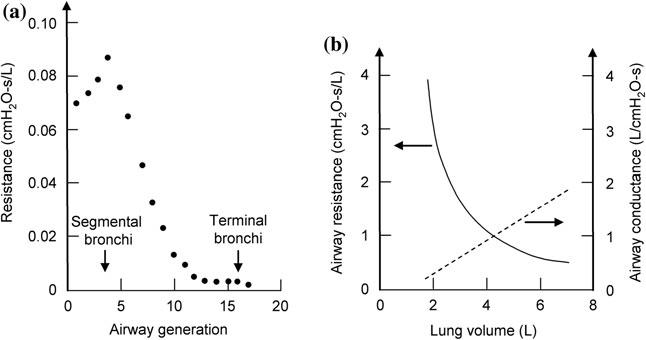
\includegraphics[width=0.8\textwidth]{914.png}
  \caption{a Resistencia de las vías respiratorias para cada generación de bronquios, y b resistencia y conductancia totales de las vías respiratorias en función del volumen pulmonar (Basado en \cite{42}, de a \cite{25}, b \cite{2}).}
  \label{fig:9.14}
\end{figure}



Esta resistencia de las vías respiratorias es aproximadamente el $80\%$ de la resistencia pulmonar total. El otro $20\%$ se debe a las fuerzas viscosas en el movimiento del tórax y de la pared pulmonar, y esto se denomina resistencia tisular.

Las propiedades elásticas de la caja torácica (junto con la pared torácica) son importantes en la respiración, al igual que las de los pulmones. La Figura 9.15 muestra el volumen de los pulmones, de las paredes torácicas solas y de los pulmones en la pared torácica como función de la presión. Esto se mide después de la inspiración o la espiración con un espirómetro y la posterior relajación de los músculos respiratorios. En cada volumen, la presión (la presión de relajación) de la combinación de pulmón/pared torácica es la suma de aquellas para los pulmones y las paredes torácicas por separado.

\begin{SCfigure}[0.9][htbp]
  \centering
  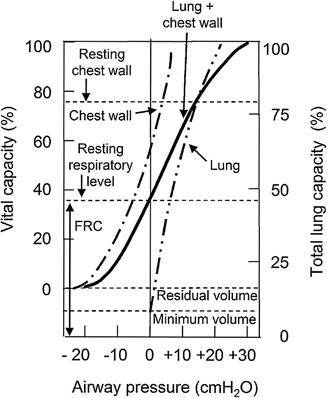
\includegraphics[width=0.5\textwidth]{915.png}
  \caption{Curvas presión-volumen de los pulmones, la pared torácica (sin pulmones) y la pared torácica con pulmones, con los músculos respiratorios relajados. Los datos pulmonares son los mismos que los de la Fig. 9.12, excepto que no se muestra histéresis y la presión de las vías respiratorias es del signo opuesto a la presión alrededor del pulmón. CRF es la capacidad residual funcional. La medición se realiza con un aparato similar a un espirómetro, parecido al de la Fig. 9.13b (Basado en \cite{42}).}
  \label{fig:9.15}
\end{SCfigure}



Con la edad avanzada, la compliancia pulmonar parece aumentar en personas sanas, pero las compliancias de la pared torácica y del sistema respiratorio total disminuyen (y esto último aumenta el trabajo respiratorio, como veremos más adelante). No hay cambios aparentes en la resistencia de las vías respiratorias \cite{32, 37}.

¿Cuáles son las presiones espiratorias e inspiratorias máximas? Para hombres jóvenes sanos, la presión manométrica promedio desarrollada durante la espiración es de $\sim 100$--$150\text{ cmH}_2\text{O}$ ($\sim 0.097$--$0.145\text{ atm}$) y durante la inspiración es de $\sim -95$ a $-105\text{ cmH}_2\text{O}$ (que también se denomina presión de inspiración de $\sim 95$--$105\text{ cmH}_2\text{O}$), y para de mujeres jóvenes sanas es de $\sim 60$--$95\text{ cmH}_2\text{O}$ durante la espiración y de $\sim -65$ a $-75\text{ cmH}_2\text{O}$ durante la inspiración \cite{15, 44}. Existe un rango muy amplio en estas presiones máximas promedio (incluso muy fuera del rango aquí reportado), dependiendo del grupo de edad y del método de medición específico, y además existe una gran dispersión entre individuos del mismo grupo incluso cuando se utiliza el mismo método. En cualquier caso, estas presiones espiratorias e inspiratorias extremas son respectivamente muy útiles para inflar globos y succionar líquidos a través de pajillas muy largas. (¿Cuál es la pajilla más larga que se puede usar? Ver el Problema 9.27).

¿Es la diferencia de presión entre los alvéolos y la atmósfera lo suficientemente grande como para impulsar la cantidad adecuada de aire hacia nuestros pulmones en cada respiración? (En condiciones normales, más vale que lo sea). Durante cada respiración, esta diferencia de presión comienza en cero, aumenta hasta un máximo $\Delta P_{\text{max}}$ y luego disminuye nuevamente a cero al final de la respiración. Determinemos la diferencia de presión promedio en esta secuencia. Modelaremos la inhalación como un medio ciclo de una onda senoidal con: $\Delta P(t) = \Delta P_{\text{max}} \sin(2\pi f t) = \Delta P_{\text{max}} \sin(\pi t / T_{\text{half period}})$, que dura un tiempo de medio ciclo $T_{\text{half period}} = 1/(2f)$. (El parámetro $f$ es igual a la frecuencia respiratoria solo si los tiempos de inhalación y espiración son iguales). Para $f = 0.25\text{ Hz}$, $T_{\text{half period}} = 2\text{ s}$. La diferencia de presión promedio durante esta inhalación es
\begin{equation}
\Delta P_{\text{av}} = \frac{1}{T_{\text{half period}}} \int_{0}^{T_{\text{half period}}} \Delta P_{\text{max}} \sin\left(\frac{\pi t}{T_{\text{half period}}}\right) dt \label{eq:9.11}
\end{equation}
\begin{equation}
\Delta P_{\text{av}} = \frac{\Delta P_{\text{max}}}{T_{\text{half period}}} \frac{T_{\text{half period}}}{\pi} \left( -\cos\left(\frac{\pi T_{\text{half period}}}{T_{\text{half period}}}\right) + \cos(0) \right) = \frac{2}{\pi} \Delta P_{\text{max}}, \label{eq:9.12}
\end{equation}

por lo que para $\Delta P_{\text{max}} = 1.1\text{ mmHg}$, vemos que $\Delta P_{\text{av}} = 0.7\text{ mmHg}$.

Supongamos que la entrada de aire por respiración es $V_{\text{in}}$. Entonces la tasa de flujo promedio es $Q_{\text{av}} = V_{\text{in}} / T_{\text{half period}}$. Para $V_{\text{in}} = 0.5\text{ L}$, esto es $0.25\text{ L/s}$. Si la tasa de flujo es proporcional a la caída de presión, $Q$ y $\Delta P$ tienen la misma dependencia del tiempo y, por lo tanto, $Q_{\text{max}} = (\pi/2)Q_{\text{av}}$, lo cual es $(\pi/2)0.25\text{ L/s} = 0.4\text{ L/s}$, y $Q(t) = Q_{\text{max}} \sin(2\pi f t) = Q_{\text{max}} \sin(\pi t / T_{\text{half period}})$. Además, $Q = \Delta P / R_{\text{flow}}$, donde $R_{\text{flow}}$ es la resistencia total al flujo en los conductos nasales, la tráquea, etc. La resistencia al flujo es $R_{\text{flow}} = \Delta P / Q$, por lo que utilizando los valores promedio vemos que $R_{\text{flow}} = 0.7\text{ mmHg}/(0.25\text{ L/s}) = 3.7 \times 10^5\text{ Pa}\cdot\text{s/m}^3$.

¿Es el flujo laminar o turbulento? Si la tráquea tiene un radio de $9\text{ mm}$, el aire fluye a una velocidad máxima $u_{\text{max}} = Q_{\text{max}}/A = (400\text{ cm}^3\text{/s})/(\pi(0.9\text{ cm})^2) = 160\text{ cm/s}$. El número de Reynolds (7.11) es $Re = \rho u d / \eta$. Utilizando la densidad de masa del aire a la temperatura corporal $\rho = 1.16 \times 10^{-3}\text{ g/cm}^3$ y la viscosidad del aire $2 \times 10^{-5}\text{ Pa}\cdot\text{s} = 2 \times 10^{-5}\text{ (N/m}^2\text{)s}$, encontramos que $Re = (1.16 \times 10^{-3}\text{ g/cm}^3)(160\text{ cm/s})(1.8\text{ cm}) / (2 \times 10^{-4}\text{ (dina/cm}^2\text{)s}) = 1,600$, por lo que generalmente se esperaría que el flujo sea laminar en la tráquea, así como en los conductos nasales internos y la faringe. Sin embargo, se espera cierta turbulencia debido a que las paredes de estos conductos no son lisas.

El flujo de aire a través de la nariz también es interesante. Debido a que nuestras narices sobresalen del cráneo con las fosas nasales en la parte inferior, el aire que inspiramos golpea el interior de la nariz y cambia su trayectoria en $90^\circ$. Durante este flujo turbulento hacia el interior de la nariz, el aire entra en contacto con las membranas mucosas que recubren el interior de la nariz y el aire inspirado de baja humedad se satura de agua, lo cual es necesario para que los pulmones no se sequen. El flujo a través de la nariz también limpia el aire mediante los vellos nasales y ayuda a calentar el aire antes de que llegue a los pulmones. Sin embargo, esta resistencia adicional hace que los pulmones trabajen más (ver más abajo). La turbulencia durante la espiración ayuda a que las membranas recuperen gran parte del vapor de agua del aire, de modo que el cuerpo no pierda mucha agua durante el reposo y también durante períodos de gran actividad, cuando las tasas de flujo de aire son mucho mayores \cite{7, 16}.

\subsection{Modelo Mecánico de la Respiración y Parámetros del Modelo} \label{subsec:9.5.2}

Acabamos de examinar únicamente la resistencia al flujo durante la respiración. La Figura 9.16b muestra un modelo mecánico más completo de los pulmones y la respiración. Es un vaso de compliancia descrito por $V(t) = V_d + C_{\text{flow}} P(t)$, atribuido a la elasticidad de los pulmones, en serie con un elemento inercial. Están en paralelo con un elemento resistivo, atribuido a la resistencia de las vías respiratorias que acabamos de examinar. Estos elementos del modelo son impulsados por una presión determinada por los músculos inspiratorios.

\begin{figure}[htbp]
  \centering
  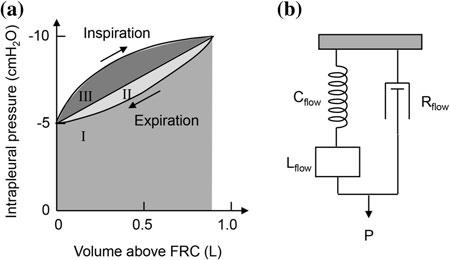
\includegraphics[width=0.8\textwidth]{916.png}
  \caption{a Trabajo realizado durante la inspiración (áreas I + II + III) y trabajo recuperado durante la espiración (área I). Sin fuerzas viscosas y resistivas, el trabajo para inflar el pulmón sería las áreas I + II, lo cual está asociado con la compliancia pulmonar. El trabajo adicional realizado para superar la resistencia al flujo respiratorio es el área III. b El modelo mecánico de la respiración tiene la compliancia concentrada (elastancia) $C_{\text{flow}}$, la resistencia $R_{\text{flow}}$ y la inertancia $L_{\text{flow}}$, y $P$ representa los músculos inspiratorios. La inertancia se puede despreciar excepto para flujos grandes (Basado en \cite{12, 41}).}
  \label{fig:9.16}
\end{figure}



\subsection{Ciclo de Inspiración/Espiración} \label{subsec:9.5.3}

La Figura 9.17 muestra la presión pulmonar, la tasa de flujo de aire hacia los pulmones y el volumen pulmonar en función del tiempo durante un ciclo de inspiración y espiración. Si el efecto de la resistencia de las vías respiratorias se omitiera, la presión alveolar sería cero y la presión intrapleural seguiría la curva discontinua, la cual está determinada por el retroceso elástico del pulmón.

\begin{figure}[htbp]
  \centering
  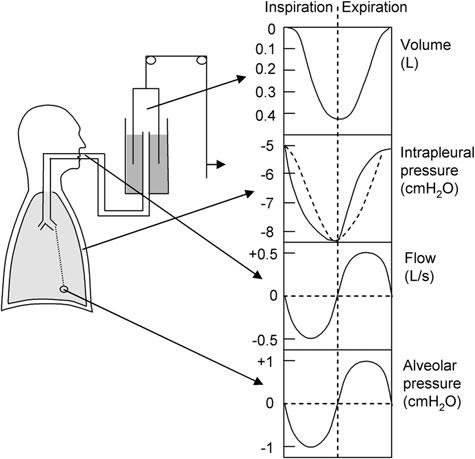
\includegraphics[width=0.55\textwidth]{917.png}
  \caption{Volumen pulmonar, presión intrapleural, flujo y presión alveolar en función del tiempo durante un ciclo respiratorio. Si se omitiera el efecto de la resistencia de las vías respiratorias, la presión alveolar sería cero y la presión intrapleural seguiría la curva discontinua (Basado en \cite{42}).}
  \label{fig:9.17}
\end{figure}



También es instructivo graficar estas variables unas en función de otras. El volumen pulmonar se grafica en función de la presión pulmonar para todos los momentos de un ciclo respiratorio en las trayectorias cíclicas discontinuas de la Fig. 9.18. El tiempo es una variable implícita a lo largo de las trayectorias. Estas gráficas son útiles porque el modelo de los pulmones incluye un vaso de compliancia en el cual el volumen y la presión están interrelacionados. Las diferencias en los diversos modos de respiración se observan fácilmente en dichas gráficas.

\begin{SCfigure}[1.0][htbp]
  \centering
  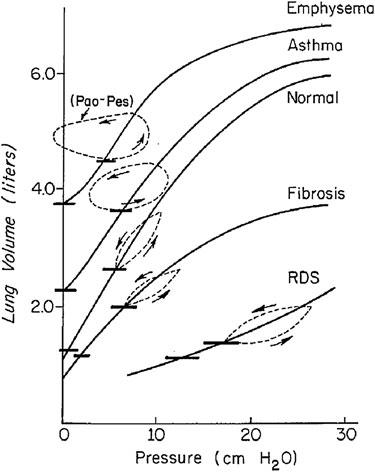
\includegraphics[width=0.45\textwidth]{918.png}
  \caption{Volumen pulmonar típico en función de la presión para pacientes con diversas condiciones respiratorias. Las curvas monótonamente crecientes son para condiciones estáticas, siendo la barra horizontal inferior el volumen residual y la barra horizontal superior la capacidad residual funcional. Se muestran lazos de respiración dinámica representativos (curvas discontinuas cerradas) para la respiración de volumen corriente ($V_T$) para cada condición (Reimpreso de \cite{12}, con permiso de Elsevier).}
  \label{fig:9.18}
\end{SCfigure}



% Control de Calidad: 17 párrafos origen -> 17 párrafos salida. Mapeo 1:1 verificado. Sin omisiones.

\subsection{Respiración con un Pulmón Enfermo} \label{subsec:9.5.4}

Las curvas estáticas y dinámicas de presión-volumen en la Fig. 9.18 indican cómo las diferentes enfermedades afectan la compliancia pulmonar, el volumen pulmonar y la resistencia de las vías respiratorias. Los trastornos obstructivos se deben a obstrucciones de las vías respiratorias que aumentan la resistencia de las vías respiratorias y limitan la espiración a frecuencias respiratorias rápidas. Incluyen la bronquitis crónica (producción excesiva de moco en el árbol bronquial), el enfisema (agrandamiento de los espacios aéreos después del bronquiolo terminal, con la destrucción de las paredes del sistema respiratorio, como las de los alvéolos) y el asma (estrechamiento generalizado de las vías respiratorias, a veces de forma espontánea). Dichas obstrucciones (Fig. 9.19) pueden deberse a secreciones excesivas (causadas por la bronquitis crónica), engrosamiento de las paredes de las vías respiratorias (edema o hipertrofia muscular) y anomalías externas (edema, ganglios linfáticos agrandados o destrucción del tejido de los alvéolos pulmonares como en el enfisema). (El edema es una acumulación excesiva de líquido en los espacios tisulares o en una cavidad corporal). Estas obstrucciones y la pérdida de vías respiratorias pequeñas debido a la destrucción del tejido pulmonar aumentan la resistencia de las vías respiratorias. La degradación de las paredes elásticas de los alvéolos también reduce la elasticidad y, por lo tanto, también la compliancia. Los trastornos restrictivos son aquellos en los que la expansión del pulmón está restringida. La disminución de la compliancia (pendiente) en la fibrosis pulmonar y en el síndrome de dificultad respiratoria idiopática (SDR) es evidente en la Fig. 9.18. Se caracterizan por una menor capacidad vital, pero la resistencia de las vías respiratorias (por volumen pulmonar) no aumenta.

\begin{figure}[htbp]
  \centering
  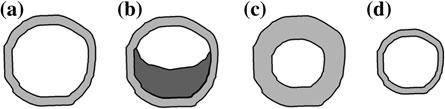
\includegraphics[width=0.8\textwidth]{919.png}
  \caption{a Vía respiratoria normal y vías respiratorias obstruidas debido a b bloqueo, c engrosamiento de la pared de la vía respiratoria y d anomalía externa. Ver también la Fig. 9.22 (Basado en \cite{41}).}
  \label{fig:9.19}
\end{figure}



La respiración deficiente debido a un pulmón enfermo se manifiesta de diferentes maneras. Como se ve en la Fig. 9.20, el volumen inspirado es muy bajo si la compliancia es menor que la normal y/o la resistencia de las vías respiratorias es mayor que la normal. También se puede utilizar un espirómetro con baja resistencia para evaluar disfunciones pulmonares de una manera ligeramente diferente a la utilizada en la Fig. 9.13. Después de una inhalación muy profunda, la persona expulsa el aire lo más rápido posible. El volumen total exhalado es la capacidad vital forzada (CVF), que puede ser un poco menor que la capacidad vital medida con una espiración más lenta. También cabe destacar el volumen exhalado en el primer $1\text{ s}$, que es el volumen espiratorio forzado (VEF) (o $\text{VEF}_1$, que denota específicamente que este volumen se espiró en $1\text{ s}$), y la relación $\text{VEF/CVF}$. Como se ve en la Fig. 9.21, para un pulmón normal, $\text{CVF} = 5.0\text{ L}$ y $\text{VEF/CVF} = 80\%$. El ejemplo de un patrón obstructivo tiene una $\text{CVF}$ menor, $3.1\text{ L}$, y una relación $\text{VEF/CVF}$ menor, $42\%$. El ejemplo de un patrón restrictivo también tiene una $\text{CVF}$ menor, $3.1\text{ L}$, pero una relación $\text{VEF/CVF}$ alta, $90\%$. Las tasas de flujo para el patrón obstructivo también son anormalmente bajas (Problema 9.31).

\begin{SCfigure}[0.8][htbp]
  \centering
  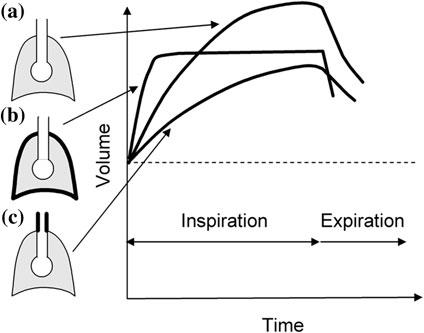
\includegraphics[width=0.55\textwidth]{920.png}
  \caption{Volumen pulmonar durante la inspiración para a condiciones normales, b compliancia disminuida y c resistencia de las vías respiratorias aumentada (Basado en \cite{42}).}
  \label{fig:9.20}
\end{SCfigure}

\begin{figure}[htbp]
  \centering
  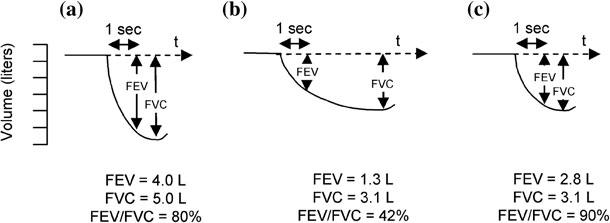
\includegraphics[width=0.8\textwidth]{921.png}
  \caption{Espiración forzada para patrones a normal, b obstructivo y c restrictivo (Basado en \cite{41}).}
  \label{fig:9.21}
\end{figure}



La Figura 9.18 muestra ciclos que tipifican los ciclos respiratorios de una persona normal y de personas con trastornos pulmonares. Las divisiones entre los alvéolos se degradan en las personas con enfisema. Como consecuencia, los pulmones se vuelven menos elásticos y más compliantes, y la contribución de la resistencia de las vías respiratorias domina la respiración. En la fibrosis pulmonar, la compliancia se reduce por un aumento del tejido fibroso. Esta condición aumenta en el enfisema pulmonar y en el envejecimiento normal, debido a un cambio en el tejido elástico de los pulmones. También se muestra el lugar geométrico volumen/presión para el síndrome de dificultad respiratoria (SDR) idiopático. Se observa que se desplaza hacia una presión más alta debido a la falta de surfactante en los alvéolos, como ocurre en algunos bebés prematuros. En tales bebés, la tensión superficial mínima es de solo $2 \times 10^{-4}\text{ N/m}$, en comparación con $\ll 0.5 \times 10^{-4}\text{ N/m}$ para pulmones normales. Con menos surfactante, la tensión superficial del alvéolo disminuye y, a la misma diferencia de presión, el alvéolo es más pequeño. La Figura 9.22 muestra que las vías respiratorias tienden a colapsar en el enfisema debido a la pérdida de tracción radial con las estructuras externas, mientras que en la fibrosis intersticial las vías respiratorias pueden llegar a tener un gran diámetro debido a la tracción radial excesiva, haciendo que las vías respiratorias sean grandes en volumen en relación con los pulmones.

\begin{SCfigure}[0.75][htbp]
  \centering
  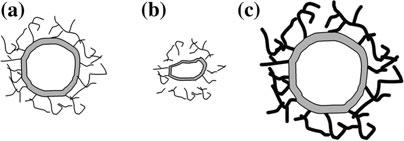
\includegraphics[width=0.6\textwidth]{922.png}
  \caption{Dimensiones de las vías respiratorias para diferentes pacientes (Basado en \cite{41}). a Normal, b Enfisema, c Fibrosis}
  \label{fig:9.22}
\end{SCfigure}



\subsection{Respiración a Altitudes Más Elevadas y Bajo Otras Condiciones Inusuales} \label{subsec:9.5.5}

La presión parcial de oxígeno es de $161\text{ mmHg}$ ($21.2\text{ kPa}$) a nivel del mar ($300\text{ K}$), lo que corresponde a un contenido de $\text{O}_2 \simeq 20.9\%$. Las personas sanas comienzan a sufrir efectos adversos para la salud a medida que la fracción de $\text{O}_2$ cae cada vez más por debajo del $19.5\%$ en la atmósfera normal a nivel del mar \cite{23, 29}. A medida que esta fracción disminuye al $10\%$, el cuerpo responde aumentando las frecuencias respiratorias (taquipnea) y las frecuencias de los latidos cardíacos (taquicardia) para incrementar el consumo de oxígeno, mientras sufre un deterioro cada vez mayor de la atención, el pensamiento y la coordinación; estas respuestas se desencadenan a niveles de esfuerzo cada vez más bajos. La respiración de aire con fracciones de oxígeno en el rango de 6--10\% produce náuseas, vómitos, movimientos letárgicos y, tal vez, pérdida del conocimiento. Respirar aire que contiene menos del 6\% de oxígeno produce convulsiones, luego el cese de la respiración (apnea), seguido por el cese de las contracciones ventriculares y la expulsión de sangre por el corazón (paro cardíaco). Este umbral crítico se llama hipoxia (que es la falta de oxígeno que llega a los tejidos vivos) y ocurre por debajo de una presión parcial crítica de $\simeq 57\text{ mmHg}$ ($7.5\text{ kPa}$) para una frecuencia respiratoria normal y relajada. (Otra forma de decir todo esto es: nuestros cuerpos han sido diseñados de modo que nuestra frecuencia de respiración de aire, la tasa de transferencia de oxígeno a la sangre, la capacidad de la sangre para retener oxígeno, las tasas de flujo sanguíneo a los tejidos, etcétera, conducen a un metabolismo que funciona bien cuando la presión parcial de oxígeno está razonablemente por encima de este valor crítico).

% Control de Calidad: 4 párrafos origen -> 4 párrafos salida. Mapeo 1:1 verificado. Sin omisiones.

Estos efectos pueden ocurrir a la presión atmosférica del nivel del mar cuando el suministro de aire no se renueva, por lo que la fracción de oxígeno disminuye (como en habitaciones selladas y automóviles sin suficiente aire fresco de renovación y en burbujas en botes volcados (ver el Problema 9.42, que también aborda el efecto del aumento de las fracciones de $\text{CO}_2$)) y cuando la fracción de oxígeno permanece esencialmente normal pero la presión parcial de $\text{O}_2$ es menor que la normal debido a la menor presión atmosférica a grandes alturas. (El cuerpo puede adaptarse solo un poco a disminuciones a largo plazo en el oxígeno disponible a mayores alturas). ¿A qué altura sobre el nivel del mar ocurre la hipoxia?

La presión de una columna de fluido de densidad de fluido constante $\rho$ y aceleración de la gravedad constante $g$ viene dada por (2.48), $P = \rho gh$, donde $h$ es la altura de la columna. En el Cap. 8 consideramos una columna de sangre; ahora consideremos una columna de aire a una altura $z$ y superior, donde $z = 0$ al nivel del mar. El cambio de presión para un cambio de altura es
\begin{equation}
dP = -\rho g dz. \label{eq:9.13}
\end{equation}

Debido a que consideraremos alturas sobre el nivel del mar que son mucho menores que el radio de la Tierra, hemos ignorado la dependencia de la aceleración de la gravedad $g$ con respecto a $z$. (Esto se considera en el Problema 9.43).

La ley de los gases ideales (7.2) es $P = nRT$, donde $n$ es la densidad, $R$ es la constante de los gases y $T$ es la temperatura, o bien
\begin{equation}
P = \frac{RT}{m} \rho, \label{eq:9.14}
\end{equation}
donde $\rho = mn$ es la densidad de masa, siendo $m$ la masa molecular. Supondremos que la temperatura atmosférica ($300\text{ K}$) no varía con la altura (ver el Problema 9.48). Dividiendo (9.13) y (9.14) se obtiene
\begin{equation}
\frac{dP}{P} = -\frac{mg}{RT} dz. \label{eq:9.15}
\end{equation}

Integrando desde el nivel del mar, $z = 0$ con presión $P_{\text{sea level}}$, hasta una altura $h$, con presión $P(h)$, se obtiene
\begin{equation}
P(h) = P_{\text{sea level}} \exp \left( -\frac{mg}{RT} h \right). \label{eq:9.16}
\end{equation}

Usando la presión parcial de oxígeno al nivel del mar y $m = 32\text{ g/mol}$ para el oxígeno, esto muestra que la hipoxia ocurre a una altura de $8.25\text{ km}$ ($= 27{,}100\text{ ft} = 5.1\text{ millas}$). (La altura del monte Everest es de $29{,}029\text{ ft}$).

\FloatBarrier
\section*{9.6 Trabajo necesario para respirar}

Durante la inspiración, el tórax y el abdomen realizan un trabajo positivo para expandir los pulmones \cite{1, 12, 18, 42}. El cuerpo no realiza ningún trabajo durante la espiración normal, pero durante la respiración forzada también se realiza trabajo para contraer los pulmones durante la espiración. Dado que $V = V_d + C_{\text{flow}} P$, para el ciclo respiratorio con el volumen cambiando entre el volumen de la capacidad residual funcional, $V_{\text{FRC}}$, y este más el volumen corriente, $V_{\text{FRC}} + V_t$, podemos escribir $V(t) = V_{\text{FRC}} + C_{\text{flow}} P(t)$. Vemos que $\Delta V(t) = V(t) - V_{\text{FRC}} = C_{\text{flow}} P(t)$ o $P(t) = \Delta V(t)/C_{\text{flow}}$. El trabajo realizado al inhalar un volumen corriente $V_t$ es
\begin{equation}
W = \int_{0}^{V_t} P d(\Delta V) = \int_{0}^{V_t} \frac{\Delta V}{C_{\text{flow}}} d(\Delta V) = \frac{V_t^2}{2C_{\text{flow}}}. \label{eq:9.17}
\end{equation}

En la Fig. 9.16a, el trabajo realizado para superar estos efectos elásticos (de compliancia) es el área definida por las regiones I + II, y esto es lo que hemos derivado aquí (y usaremos más adelante). El trabajo es en realidad mayor, el área representada por las regiones I + II + III, debido a los efectos viscosos (resistivos). (Estos efectos viscosos/resistivos también conducen a la histéresis aquí y en la Fig. 9.12, tal como en el Cap. 4).

Para una frecuencia respiratoria $f$, la tasa de realización de trabajo para la inspiración es
\begin{equation}
\frac{dW}{dt} = f \frac{V_t^2}{2C_{\text{flow}}}. \label{eq:9.18}
\end{equation}

Con una frecuencia respiratoria de $20/\text{min}$, un volumen corriente de $500\text{ cm}^3$ y una compliancia pulmonar de $0.1\text{ L/cmH}_2\text{O} = 0.1\text{ cm}^3/(\text{dina/cm}^2)$, esto es
\begin{equation}
\frac{dW}{dt} = \frac{(20/\text{min})(500\text{ cm}^3)^2}{2 \times 0.1\text{ cm}^3/(\text{dina/cm}^2)} = 3.6 \times 10^3\text{ J/día} = 0.86\text{ kcal/día}. \label{eq:9.19}
\end{equation}

La eficiencia de los músculos respiratorios es $\epsilon = 5\text{--}10\%$, por lo que la necesidad metabólica es
\begin{equation}
\frac{dE}{dt} = \frac{dW/dt}{\epsilon} = \frac{0.86\text{ kcal/día}}{0.05} = 17\text{ kcal/día} \label{eq:9.20}
\end{equation}
asumiendo una eficiencia del $5\%$; este cálculo es muy sensible a los valores elegidos para $C_{\text{flow}}$ y $\epsilon$. Este resultado es aproximadamente el $1\%$ de la Tasa Metabólica Basal (BMR); sin embargo, este valor es en realidad de alrededor del $2\%$ de la BMR, por lo que tal vez $\epsilon$ esté más cerca del $3\%$ y/o sea necesario considerar otros efectos, como la disipación debida a la resistencia del flujo y la naturaleza viscosa (de la viscoelasticidad general) de los pulmones y la pared torácica. La resistencia al flujo de aire en la nariz parece ser responsable de aproximadamente la mitad del trabajo necesario para respirar.

Durante la respiración normal no se realiza trabajo mecánico en la espiración. Durante los entrenamientos pesados y el ejercicio extenuante, las necesidades metabólicas aumentan porque (1) también se realiza trabajo durante la espiración, (2) la frecuencia respiratoria es más rápida y (3) el volumen corriente es mayor. El trabajo realizado para respirar puede entonces consumir el $25\%$ del consumo total de energía del cuerpo. Un aumento tan grande se sugiere en la Fig. 8.26. La respiración rápida y superficial (como se recomienda en el entrenamiento de Lamaze para el parto) requiere más energía que la respiración normal, para superar la naturaleza resistiva del flujo en los pasajes de aire. Del mismo modo, la respiración lenta y profunda requiere más energía para superar la naturaleza elástica del pulmón y del tórax. El Problema 9.12 compara otras ventajas y desventajas relativas de estos dos últimos modos de respiración.

Otra cosa interesante puede ocurrir durante la espiración forzada. En la respiración normal, la presión en las vías respiratorias siempre excede la presión intrapleural durante la inspiración y la espiración (como se ve en la Fig. 9.23 durante la inspiración normal). Sin embargo, durante la espiración forzada, tanto la presión intrapleural como la de los alvéolos aumentan en la misma cantidad ($38\text{ cmH}_2\text{O}$) y, por lo tanto, ambas son positivas con respecto a la atmósfera ($+30$ y $+38\text{ cmH}_2\text{O}$ en la figura). Hay entonces una gran caída de presión desde los alvéolos hasta los labios y las fosas nasales. En algún punto a lo largo de esta ruta, la presión en las vías respiratorias será inferior a $30\text{ cmH}_2\text{O}$ y esto comprimirá las vías respiratorias (que se muestra donde la presión es $+19\text{ cmH}_2\text{O}$ en esta figura) y aumentará la resistencia de las vías respiratorias.

\begin{figure}[htbp]
  \centering
  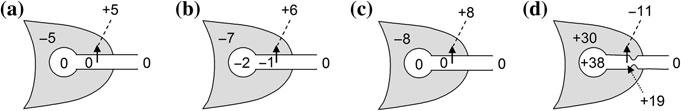
\includegraphics[width=0.8\textwidth]{923.png}
  \caption{Presiones intrapleurales, de los alvéolos, de las vías respiratorias y atmosféricas en $\text{cmH}_2\text{O}$ durante la inspiración y la espiración forzada (Basado en \cite{42}). \textbf{a}~Preinspiración, \textbf{b}~Durante la inspiración, \textbf{c}~Fin de la inspiración, \textbf{d}~Espiración forzada.}
  \label{fig:9.23}
\end{figure}



\FloatBarrier
\section*{9.7 Resumen}

La base macroscópica de la función pulmonar y la respiración se puede entender analizando el volumen, la presión y el flujo de aire durante la respiración, utilizando modelos de flujo de fluidos y expansión pulmonar. La naturaleza física de las unidades de funcionamiento individuales en los pulmones, es decir, los alvéolos, también se puede entender de esta manera. Estos modelos también se pueden usar para comprender las consecuencias físicas de un pulmón enfermo. La energía necesaria para hacer funcionar los pulmones también se puede modelar.

% Control de Calidad: 18 párrafos origen -> 18 párrafos salida. Mapeo 1:1 verificado. Sin omisiones.

\FloatBarrier
\clearpage
\section*{Problemas}

\subsection*{Pulmones}

\noindent \textbf{9.1} Calcule los volúmenes pulmonares efectivos y las frecuencias respiratorias para un hombre ($70\text{ kg}$), una mujer ($50\text{ kg}$) y un lactante ($5\text{ kg}$) usando los parámetros de la relación alométrica de la Tabla 1.13. ¿Cómo se comparan las frecuencias respiratorias con las dadas anteriormente?

\noindent \textbf{9.2} Si hay $3 \times 10^8$ alvéolos en un pulmón con una capacidad residual funcional (FRC) de $2.5\text{ L}$, calcule el volumen y el radio promedio de un alvéolo.

\noindent \textbf{9.3} Use la Tabla 9.1 para demostrar que el aire viaja una distancia total de $273\text{ mm}$ desde la tráquea hasta los alvéolos.

\noindent \textbf{9.4} ¿Cuál es el volumen total de los pulmones descritos en la Tabla 9.1? ¿Dónde se encuentra la mayor parte del volumen?

\noindent \textbf{9.5} ¿Se cumple la continuidad del flujo con los datos para los pulmones en la Tabla 9.1? Verifique esto utilizando los datos para las generaciones bronquiales 0, 1, 2, 3, 4, 5, 10, 16, 20 y 23.

\noindent \textbf{9.6} Calcule el número de Reynolds para las generaciones bronquiales enumeradas en el Problema 9.5. ¿Es el flujo laminar o turbulento en el sistema respiratorio?

\noindent \textbf{9.7} Calcule la caída de presión a través de los órdenes arteriales pulmonares 1, 4, 10, 13, 16 y 17, asumiendo un flujo sanguíneo total de $5\text{ L/min}$.

\noindent \textbf{9.8} El nivel de $\text{CO}_2$ en la atmósfera era de $\sim 280\text{ ppm}$ (partes por millón) en la época preindustrial y es de $\sim 380\text{ ppm}$ ahora (2015). Exprese estos niveles en términos de $\text{mmHg}$. ¿Se esperaría que este cambio afecte el intercambio de $\text{CO}_2$ en los pulmones de alguna manera significativa?

\subsection*{Alvéolos y tensión superficial}

\noindent \textbf{9.9} Derive (9.8) a partir de (9.7).

\noindent \textbf{9.10} Estime la fuerza que tendría que ejercer el diafragma adulto si no hubiera surfactante pulmonar.

\subsection*{Respiración}

\noindent \textbf{9.11} Use la Fig. 9.13b para explicar cómo funciona un espirómetro. ¿Cuánto debería subir y bajar el agua en el espirómetro durante los ciclos respiratorios? (Asuma dimensiones razonables para el instrumento).

\noindent \textbf{9.12} Durante la respiración, la ventilación pulmonar, $V_p$ (en $\text{L/min}$) (la tasa a la que el aire ingresa a la tráquea), es igual a la frecuencia respiratoria, $R$ (en unidades de por minuto), multiplicada por el volumen corriente, $V_t$ (en $\text{L}$). Debido al volumen de espacio muerto anatómico $V_d$, solo $V_t - V_d$ ingresa a los alvéolos (y, por lo tanto, es de utilidad). Por lo tanto, una tasa de ventilación más significativa es la ventilación alveolar $V_a = R(V_t - V_d)$:
\par\noindent (a) Encuentre $V_p$ y $V_a$ para las condiciones en la Tabla 9.3, asumiendo $V_d = 0.15\text{ L}$.
\par\noindent (b) Compare la ventilación pulmonar para los cuatro patrones respiratorios en esta tabla para la persona en reposo. (Los patrones (ii) a (iv) requieren más potencia metabólica que el (i), debido al aumento del trabajo por la resistencia al flujo y la resistencia en los tejidos para (ii) y (iii), y al aumento del trabajo por las fuerzas de compliancia (elásticas) del pulmón y del tórax en (iv)). ¿Cuál de los cuatro es claramente desaconsejable debido a una mala ventilación alveolar?
\par\noindent (c) Durante el ejercicio, tanto la frecuencia respiratoria como el volumen corriente aumentan. Con base en los resultados de la parte (a) para (i) a (iv) y para (v) a (vi), ¿se gana más respirando más rápido o más profundo para una ventilación pulmonar dada?

\noindent \textbf{9.13} ¿Cuáles son los flujos de aire máximo y promedio para cada ciclo respiratorio en el Problema 9.12, asumiendo que los períodos de inhalación y exhalación son los mismos?

\noindent \textbf{9.14} (a) Cuando realiza una inspiración profunda de, por ejemplo, $1\text{ L}$, ¿cuánto aumentan su masa (en $\text{kg}$) y su peso (en $\text{N}$ y $\text{lb}$)?
\par\noindent (b) ¿Su densidad promedio aumenta, disminuye o permanece igual? Si hay un cambio, estímelo.

\noindent \textbf{9.15} (a) ¿Qué dice la Fig. 8.26 sobre la cantidad de oxígeno que se puede consumir por cantidad de gasto cardíaco?
\par\noindent (b) ¿Qué dice sobre cuánto oxígeno se necesita para realizar un trabajo? ¿Es esto consistente con lo que se presenta en el texto?
\par\noindent (c) ¿Cómo se define la salida de trabajo en esta figura?

\noindent \textbf{9.16} Estime la resistencia de la tráquea usando la ley de Poiseuille, asumiendo que tiene un radio de $9\text{ mm}$ y una longitud de $110\text{ mm}$. ¿Cómo se compara esto con la resistencia total?

\noindent \textbf{9.17} Estime la resistencia del tracto vocal usando la ley de Poiseuille, asumiendo que puede modelarse como tres tubos en serie con longitudes respectivas de $6$, $3$ y $6\text{ cm}$ y áreas de sección transversal de $5$, $1$ y $5\text{ cm}^2$. (También dibuje un esquema de este modelo).

\begin{table}[htbp]
  \centering
  \caption{Ejemplos de ciclos respiratorios.}
  \label{tab:9.3}
  \begin{tabularx}{\textwidth}{Xcc}
    \toprule
    Actividad & $R$ (por min) & $V_t$ ($\text{L}$) \\
    \midrule
    (i) En reposo, respiración tranquila & 12 & 0.5 \\
    (ii) En reposo, con respiración rápida y superficial & 24 & 0.25 \\
    (iii) En reposo, con respiración muy rápida y muy superficial & 40 & 0.15 \\
    (iv) En reposo, con respiración lenta y profunda & 6 & 1.0 \\
    (v) Ejercicio, con respiración rápida y superficial & 24 & 0.5 \\
    (vi) Ejercicio, con respiración lenta y profunda & 12 & 1.0 \\
    \bottomrule
  \end{tabularx}
\end{table}

\noindent \textbf{9.18} Estime la resistencia del pasaje nasal usando la ley de Poiseuille, asumiendo que tiene un radio de $4\text{ mm}$ y una longitud de $3\text{ cm}$. ¿Cómo se compara esto con la resistencia total y es un factor limitante en la resistencia al flujo?

\noindent \textbf{9.19} Si se modela la vía respiratoria como una serie de pasajes secuenciales: el pasaje nasal o bucal, la faringe, la laringe y luego la tráquea, cada uno con una resistencia al flujo de aire, ¿cuál es la resistencia total al flujo de aire en términos de estas resistencias individuales?

\noindent \textbf{9.20} Tanto en la inspiración como en la espiración, una diferencia de presión de $0.4\text{ cmH}_2\text{O}$ causa un flujo de $0.15\text{ L/s}$ en la nariz. Determine la resistencia al flujo en ella.

\noindent \textbf{9.21} Considere las generaciones de bifurcación pulmonar 1--19 en la Tabla 9.1:
\par\noindent (a) ¿En qué generación es mayor la resistencia al flujo? ¿Cuál es su valor?
\par\noindent (b) ¿Coinciden sus resultados con los de la Fig. 9.14a?
\par\noindent (c) ¿En qué generación es mayor la caída de presión y, en general, en qué rango de bifurcaciones se produce la mayor parte de la caída de presión?

\noindent \textbf{9.22} La resistencia total de las vías respiratorias es la suma de las resistencias en cada generación pulmonar. ¿Se suman las resistencias en la Fig. 9.14a para dar una resistencia total consistente con la de la Fig. 9.14b?

\noindent \textbf{9.23} Calcule la resistencia para la generación pulmonar 4 usando la ley de Poiseuille y compárela con los valores dados en el capítulo.

\noindent \textbf{9.24} Al inflar un globo, usted exhala el $80\%$ de la capacidad vital (de $4\text{ L}$) con cada respiración. ¿Cuántas respiraciones se necesitan para inflar un globo desde un volumen muy pequeño (despreciable) hasta una esfera con un diámetro de $10\text{ pulgadas}$?

\noindent \textbf{9.25} (a) Al inflar un globo, el volumen inicialmente aumenta lentamente con el aumento de la presión hasta alcanzar una presión máxima (cuando el globo está solo parcialmente inflado) y, a medida que continúa soplando, el volumen aumenta rápidamente y la presión interna disminuye. Explique por qué algunas personas pueden inflar globos fácilmente y otras no.
\par\noindent (b) En un estudio, el volumen del globo se incrementó lentamente hasta que la presión manométrica interna alcanzó $2.0 \times 10^4\text{ dyn/cm}^2$ y luego el volumen se incrementó más rápidamente, a medida que la presión interna disminuyó a $1.5 \times 10^4\text{ dyn/cm}^2$ \cite{17, 20}. ¿Esperaría poder inflar este globo (y por qué lo cree)?

\noindent \textbf{9.26} No todo el mundo tiene la misma presión espiratoria máxima. Suponga que la presión espiratoria máxima es de $100 \pm 40\text{ cmH}_2\text{O}$ para un grupo de hombres y de $60 \pm 40\text{ cmH}_2\text{O}$ para un grupo similar de mujeres. Estime la fracción de personas que son capaces de inflar un tipo de globo determinado, para el cual la presión de inflado es de $80\text{ cmH}_2\text{O}$. Asuma que hay igual número de hombres y de mujeres.

\noindent \textbf{9.27} (a) ¿Cuál es la pajilla (sorbete) para beber vertical más larga que un hombre con una presión inspiratoria máxima de $150\text{ cmH}_2\text{O}$ puede usar para beber agua (usando una sola respiración)? (Ignore las limitaciones debidas al volumen inspiratorio y a consideraciones de flujo resistivo).
\par\noindent (b) ¿Cuál es el diámetro (interno) más grande que podría tener la pajilla, dada la limitación de que la persona puede mantener esta presión solo durante el $40\%$ de la capacidad vital de $4.5\text{ L}$?

\noindent \textbf{9.28} (a) Use la Fig. 9.15 para determinar la compliancia de los pulmones ($C_{\text{flow,lung}}$) y de las paredes torácicas ($C_{\text{flow,chest wall}}$) al $0$, $20$, $40$, $60$ y $80\%$ de la capacidad vital. (b) Determine la compliancia del sistema combinado pulmón/pared torácica ($C_{\text{flow,lung/chest wall}}$) a estos volúmenes y compare estos valores con los de la parte (a) usando $1/C_{\text{flow,lung/chest wall}} = 1/C_{\text{flow,lung}} + 1/C_{\text{flow,chest wall}}$.

\noindent \textbf{9.29} (a) Use la Fig. 9.18 para determinar la compliancia de los pulmones para cada condición (dentro del rango de presión más bajo de $5\text{ cmH}_2\text{O}$ mostrado para cada una).
\par\noindent (b) ¿Cómo varía la compliancia para cada una en el rango de presión mostrado?

\noindent \textbf{9.30} Compare las compliancias pulmonares específicas de un hombre de $65\text{ kg}$ y un ratón de $20\text{ g}$, con compliancias respectivas de $0.2\text{ L/cmH}_2\text{O}$ y $0.0001\text{ L/cmH}_2\text{O}$.

\noindent \textbf{9.31} Demuestre que las tasas de flujo espiratorio forzado (FEF) para los flujos normal, obstructivo y restrictivo en la Fig. 9.21 son de $3.5$, $1.4$ y $3.7\text{ L/s}$, respectivamente. Haga esto determinando las pendientes de las tres curvas en esta figura. (Use un ajuste de línea recta entre los puntos que han disminuido entre el $25$ y el $75\%$ en camino hacia la FVC).

\noindent \textbf{9.32} Determine la resistencia al flujo de aire a partir de la tasa de flujo y la presión alveolar en la Fig. 9.17.

\noindent \textbf{9.33} Considere solo la compliancia en el trabajo de la respiración y asuma que la compliancia $C_{\text{flow}}$ para pulmones normales es de $0.1\text{ cm}^5/\text{dina}$:
\par\noindent (a) En la fibrosis pulmonar, la compliancia de los pulmones disminuye. Para un volumen corriente dado, ¿cómo cambia la tasa de trabajo de la respiración si la compliancia disminuye en un $x\%$?
\par\noindent (b) Compare la tasa de trabajo realizado al respirar ($\text{J/día}$) y la tasa de metabolismo asociada ($\text{kcal/día}$) (si los músculos asociados con la respiración tienen una eficiencia del $5\%$) para los casos (i) y (iv) en el Problema 9.12 para pulmones normales.

\noindent \textbf{9.34} (problema avanzado) Escriba la ecuación de movimiento para el modelo mecánico de la Fig. 9.16b y resuélvala para la integración de la inspiración.

\noindent \textbf{9.35} (problema avanzado) Demuestre que la solución del Problema 9.34 concuerda cualitativamente con las tendencias observadas en la Fig. 9.20: con una menor compliancia, la constante de tiempo disminuye y el volumen respirado durante un ciclo disminuye, mientras que con un aumento de la resistencia de las vías respiratorias, la constante de tiempo aumenta y el volumen respirado durante un ciclo disminuye.

\noindent \textbf{9.36} Estime la tasa de energía consumida por los pulmones durante el ejercicio con una frecuencia respiratoria de $40/\text{min}$ y un volumen corriente de $1{,}000\text{ cm}^3$.

\noindent \textbf{9.37} Use una tasa de circulación sanguínea de $5\text{ L/min}$ y el cambio conocido en las presiones parciales de $\text{O}_2$ y $\text{CO}_2$ en los capilares sistémicos para encontrar el número de litros de $\text{O}_2$ consumidos y $\text{CO}_2$ exhalados cada día. ¿Cómo cambian sus resultados si en su lugar usa el cambio en las presiones parciales de $\text{O}_2$ y $\text{CO}_2$ en los capilares pulmonares? Explique por qué.

% Control de Calidad: 37 párrafos origen -> 37 párrafos salida. Mapeo 1:1 verificado. Sin omisiones.

\noindent \textbf{9.38} Si la pared torácica y la pleura parietal de un pulmón son perforadas, la presión intrapleural aumentará hasta la presión atmosférica y ese pulmón colapsará. Explique por qué. También dibuje un diagrama explicando esto.

\noindent \textbf{9.39} (a) Cuando realiza actividades que requieren una alta tasa metabólica, como correr, a veces respira por la boca para aumentar la tasa de entrada de aire. Esto puede ocurrir, por ejemplo, cuando sus fosas nasales se contraen hacia adentro cuando intenta inspirar demasiado rápido por la nariz, lo que impide el flujo de aire. Explique por qué puede deshidratarse al respirar hacia adentro y hacia afuera por la boca y no por la nariz.
\par\noindent (b) Cuando corre, ¿sería útil inspirar por la boca (para aumentar la tasa de entrada de aire) y espirar por la nariz?

\noindent \textbf{9.40} Si todo el aire que inspira ($5\text{ L/min}$) tiene una humedad relativa de cero y se satura por completo con agua ($47\text{ mmHg}$ a la temperatura corporal) durante la inspiración, ¿cuánta agua (en $\text{L}$) perdería cada día si nada de este vapor de agua fuera recapturado durante la espiración? ¿Podría esto causar deshidratación?

\noindent \textbf{9.41} Continuemos con el Problema 9.40 calculando la tasa de pérdida de energía del cuerpo debido a la pérdida de calor de vaporización del agua durante la inspiración, sin condensación posterior durante la espiración. ¿Qué tan significativo es esto?

\subsection*{Respiración a mayores alturas y bajo otras condiciones inusuales}

\noindent \textbf{9.42} Un bote vuelca y un marinero queda atrapado en una burbuja de aire que sube a la parte superior del bote volcado mientras espera el rescate \cite{21, 35}.
\par\noindent (a) ¿Qué volumen de aire fresco a presión atmosférica inspiraría alguien como el marinero en dos días? Asuma una frecuencia respiratoria de $6\text{ L de aire/min}$. En este problema, dé todos los volúmenes en términos de $\text{m}^3$ y la longitud del cubo (en $\text{ft}$) con ese volumen.
\par\noindent (b) Supongamos que la respuesta a (a) es el volumen de esta burbuja. ¿Qué fracción del aire sería $\text{O}_2$ después de dos días si comenzó en una fracción del $20.9\%$, el marinero continúa respirando a la tasa volumétrica habitual y consume un neto de $0.3\text{ L de }\text{O}_2/\text{min}$ (lo que tiene en cuenta el $\text{O}_2$ en la espiración)? ¿Cuál es el estado del marinero después de dos días?
\par\noindent (c) Vuelva a calcular el volumen de esta burbuja después de dos días, recordando ahora que se produce una molécula de $\text{CO}_2$ por cada molécula de $\text{O}_2$ consumida. Ignore la difusión de aire a través del agua y la solubilidad del $\text{CO}_2$ en el agua.
\par\noindent (d) Demuestre que por cada $10\text{ m}$ adicionales por debajo de la superficie del agua, la presión local aumenta en $1\text{ atm}$ (el valor al nivel del mar), y luego vuelva a determinar los volúmenes de la burbuja en (a) y (c) si la burbuja se formó cuando el bote estaba al nivel del mar y luego el bote se movió a $30\text{ m}$ por debajo del nivel del mar. ¿Cómo podrían ser significativos estos volúmenes si el bote fuera pequeño?
\par\noindent (e) Cuando el nivel de $\text{CO}_2$ en el aire aumenta desde los $400\text{ ppm}$ habituales a aproximadamente el $5\%$, una persona se confunde y entra en pánico, comienza a hiperventilar y finalmente pierde el conocimiento. ¿Cuál es este porcentaje en la burbuja de aire después de dos días? (En cualquier caso, si es rescatado a tiempo, el marinero aún necesitaría pasar tiempo en una cámara de descompresión para evitar el «síndrome de descompresión» si de hecho estuviera a $30\text{ m}$ o más por debajo del nivel del mar, debido a la mayor cantidad de nitrógeno disuelto en la sangre a esta presión más alta. Si este procedimiento no se realizara, se formarían burbujas de nitrógeno en su cuerpo cuando regrese al nivel del mar, lo que podría provocar su muerte).

\noindent \textbf{9.43} (a) Demuestre que la aceleración de la gravedad $g$ varía con la altura $z$ sobre el nivel del mar como $g(z) = g (R_{\text{Earth}}/(R_{\text{Earth}} + z))^2$, donde el radio de la Tierra es $R_{\text{Earth}} = 6{,}378\text{ km}$.
\par\noindent (b) Demuestre que esta variación no afecta al análisis de la privación de oxígeno a grandes alturas, descrito en el texto.

\noindent \textbf{9.44} ¿Cuál es la presión atmosférica en la ciudad a una milla de altitud («mile-high») de Denver? ¿Cuál es la presión parcial de oxígeno allí?

\noindent \textbf{9.45} Los aviones comerciales suelen volar a una altitud de crucero de $\sim 10{,}700\text{ m}$ ($\sim 35{,}000\text{ ft}$). ¿Cuáles son la presión total y la presión parcial de oxígeno a esa altura? ¿Por qué se presurizan los aviones? ¿Por qué se dispone de máscaras de oxígeno en caso de que la cabina se despresurice?

\noindent \textbf{9.46} ¿Por qué algunos atletas entrenan a grandes alturas?

\noindent \textbf{9.47} Aplique (9.16) a la variación de la presión parcial de nitrógeno, usando $m = 28\text{ g/mol}$. Digamos aquí que la relación entre oxígeno y nitrógeno es $20.9\%/78.1\% = 0.268$ al nivel del mar. ¿Cuál es esta relación a la altura crítica para la hipoxia?

\noindent \textbf{9.48} La temperatura de la troposfera (la atmósfera hasta aproximadamente $11\text{ km}$) disminuye con la altura, un poco menos de $1\text{ K}$ por cada $100\text{ m}$ de elevación. En la atmósfera estándar $T(z) = T_{\text{sea level}} + \alpha z$, con $T_{\text{sea level}} = 288.19\text{ K}$ y $\alpha = -0.00649\text{ K/km}$. (Para una atmósfera seca, $\alpha = -0.0098\text{ K/km}$, en comparación con no tener esta consideración).
\par\noindent (a) Use esta variación de temperatura en (9.15) para demostrar que
\begin{equation}
P(h) = P_{\text{sea level}} \left( \frac{T_{\text{sea level}}}{T_{\text{sea level}} + \alpha h} \right)^{\frac{gm}{R\alpha}}. \label{eq:9.21}
\end{equation}
\par\noindent (b) Demuestre que la hipoxia ocurre a una elevación menor, $7.21\text{ km}$, que sin esta consideración.

\noindent \textbf{9.49} La Tabla 9.4 compara la presión parcial de oxígeno (en $\text{mmHg}$) en el aire y en el cuerpo al nivel del mar y a una elevación de $2{,}500\text{ m}$:
\par\noindent (a) Justifique los valores dados para la presión total y la presión parcial de $\text{O}_2$ a $2{,}500\text{ m}$.
\par\noindent (b) Justifique la presión parcial de $\text{O}_2$ en los alvéolos a $2{,}500\text{ m}$ utilizando la presión al nivel del mar.
\par\noindent (c) Al nivel del mar, su sangre fluye a una tasa de $5\text{ L/min}$. ¿Qué tan rápido tendría que fluir a una elevación de $2{,}500\text{ m}$ para proporcionar el mismo flujo de oxígeno a los tejidos? (Asuma que no hay cambios en las concentraciones de glóbulos rojos y hemoglobina en la sangre. Estas aumentan como parte de la adaptación a mayores alturas).
\par\noindent (d) ¿Qué tan rápido tendría que respirar a esta elevación (en litros de aire por minuto) para mantener la misma tasa de suministro de oxígeno? ¿Cómo podría traducirse esto en cambios en la frecuencia respiratoria y el volumen corriente?

\begin{table}[htbp]
  \centering
  \caption{Presiones totales y parciales a diferentes alturas (Utilizando datos de \cite{43}).}
  \label{tab:9.4}
  \begin{tabularx}{\textwidth}{Xcc}
    \toprule
    Altitud & Nivel del mar & A $2{,}500\text{ m}$ \\
    \midrule
    Presión atmosférica (total) & 760 & 560 \\
    Presión atmosférica ($\text{O}_2$) & 159 & 117 \\
    En los alvéolos ($\text{O}_2$) & 105 & 77 \\
    En la sangre arterial ($\text{O}_2$) & 100 & 72 \\
    En la sangre venosa ($\text{O}_2$) & 40 & 40 \\
    \bottomrule
  \end{tabularx}
\end{table}

% Control de Calidad: 12 párrafos origen -> 12 párrafos salida. Mapeo 1:1 verificado. Sin omisiones.

\FloatBarrier
\clearpage
\begin{thebibliography}{99}
\bibitem{1} G.B. Benedek, F.M.H. Villars, \textit{Physics with Illustrative Examples from Medicine and Biology}, tres volúmenes, 2.ª ed. (AIP/Springer, Nueva York/Berlín, 2000)
\bibitem{2} W.A. Briscoe, A.B. DuBois, The relationship between airway resistance, airway conductance and lung volume in subjects of different age and body size. \textit{J. Clin. Invest.} \textbf{37}, 1279--1285 (1958)
\bibitem{3} J.R. Cameron, J.G. Skofronick, R. Grant, \textit{Physics of the Body}, Medical Physics, 2.ª ed. (Madison, WI, 1999)
\bibitem{4} H.K. Chang, M. Paiva (eds.), en \textit{Respiratory Physiology: An Analytical Approach}, ed. por C. Lenfant exec. Lung Biology in Health and Disease, vol. 40 (Dekker, Nueva York, 1989)
\bibitem{5} R.G. Crystal, J.B. West, P.J. Barnes, E.R. Weibel (eds.), \textit{The Lung: Scientific Foundations}, 2.ª ed. (Lippincott-Raven, Nueva York, 1997)
\bibitem{6} M.L. Foss, S.J. Keteyian, \textit{Fox's Physiological Basis for Exercise and Sport}, 6.ª ed. (McGraw-Hill, Boston, 1998)
\bibitem{7} R.G. Franciscus, E. Trinkaus, Nasal morphology and the emergence of \textit{Homo erectus}. \textit{Am. J. Phys. Anthropol.} \textbf{75}, 517--527 (1988)
\bibitem{8} R.A. Freitas Jr., \textit{Nanomedicine}, volumen I: Basic Capabilities (Landes Bioscience, Austin, 1999)
\bibitem{9} Y.C. Fung, \textit{Biodynamics: Circulation} (Springer, Berlín, 1984)
\bibitem{10} Y.C. Fung, \textit{Biomechanics: Circulation}, 2.ª ed. (Springer, Berlín, 1997)
\bibitem{11} J.F. Green, \textit{Fundamental Cardiovascular and Pulmonary Physiology}, 2.ª ed. (Lea \& Febiger, Filadelfia, 1987)
\bibitem{12} J. Hildebrandt, Structural and mechanical aspects of respiration, en \textit{Textbook of Physiology}, 21.ª ed., editado por H.D. Patton, A.F. Fuchs, B. Hille, A.M. Scher, R. Steiner (Saunders, Filadelfia, 1989), Cap. 52, pp. 991--1011
\bibitem{13} F.C. Hoppensteadt, C.S. Peskin, \textit{Modeling and Simulation in Medicine and the Life Sciences}, 2.ª ed. (Springer, Berlín, 2002) (La primera edición de 1992 se tituló \textit{Mathematics in Medicine and the Life Sciences})
\bibitem{14} J. Keener, J. Sneyd (eds.), \textit{Mathematical Physiology II: Systems Physiology}, 2.ª ed. (Springer, Berlín, 2009)
\bibitem{15} C.G. Lausted, A.T. Johnson, W.H. Scott, M.M. Johnson, K.M. Coyne, D.C. Coursey, Maximum static inspiratory and expiratory pressures with different lung volumes. \textit{BioMed. Eng. Online} \textbf{5}, 29--34 (2006)
\bibitem{16} D.E. Lieberman, \textit{The Story of the Human Body: Evolution, Health, and Disease} (Pantheon, Nueva York, 2013)
\bibitem{17} D.R. Merritt, F. Weinhaus, The pressure curve for a rubber balloon. \textit{Am. J. Phys.} \textbf{46}, 976--977 (1978)
\bibitem{18} J. Milic-Emili, E. D'Angelo, Work of breathing, en \textit{The Lung: Scientific Foundations}, 2.ª ed., editado por R.G. Crystal, J.B. West, P.J. Barnes, E.R. Weibel (Lippincott-Raven, Nueva York, 1997), Cap. 105, pp. 1437--1446
\bibitem{19} J. Moya, L. Phillips, J. Sanford, M. Wooton, A. Gregg, L. Schuda, A review of physiological and behavioral changes during pregnancy and lactation: potential exposure factors and data gaps. \textit{J. Exposure Sci. Environ. Epidemiol.} \textbf{24}, 449--458 (2014)
\bibitem{20} I. Müller, P. Strehlow, \textit{Rubber and Rubber Balloons, Paradigms of Thermodynamics}. Lecture Notes in Physics, vol. 637 (Springer, Berlín, 2004)
\bibitem{21} R. Nuwer, Trapped in an underwater air bubble for three days. \textit{Slate}, \url{http://www.slate.com/articles/health_and_science/science/2013/06/harrison_okene_s_shipwreck_air_bubble_how_could_he_survive_underwater_for.html} (18 de junio de 2013)
\bibitem{22} G. Nucci, C. Cobelli, Mathematical models of respiratory mechanics, en \textit{Modelling Methodology for Physiology and Medicine}, editado por E. Carson, C. Cobelli (Academic, San Diego, 2001), Cap. 10, pp. 279--304
\bibitem{23} Occupational Safety and Health Administration (OSHA), \url{https://www.osha.gov/pls/oshaweb/owadisp.show_document?p_id=25743&p_table=INTERPRETATIONS}
\bibitem{24} J.T. Ottesen, M.S. Olufsen, J.K. Larsen (eds.), \textit{Applied Mathematical Models in Human Physiology} (SIAM, Filadelfia, 2004)
\bibitem{25} T.J. Pedley, R.C. Schroter, M.F. Sudlow, The prediction of pressure drop and variation of resistance within the human bronchial airways. \textit{Respir. Physiol.} \textbf{9}, 387--405 (1970)
\bibitem{26} T.J. Pedley, R.D. Kamm, Dynamics of gas-flow and pressure-flow relationships, en \textit{The Lung: Scientific Foundations}, 2.ª ed., editado por R.G. Crystal, J.B. West, P.J. Barnes, E.R. Weibel (Lippincott-Raven, Nueva York, 1997), Cap. 99, pp. 1365--1381
\bibitem{27} S.E. Rees, S. Kjaergaard, S. Andreassen, Mathematical modelling of pulmonary gas exchange, en \textit{Modelling Methodology for Physiology and Medicine}, editado por E. Carson, C. Cobelli (Academic, San Diego, 2001), Cap. 9, pp. 253--278
\bibitem{28} V.C. Rideout, \textit{Mathematical and Computer Modeling of Physiological Systems} (Prentice-Hall, Englewood Cliffs, 1991)
\bibitem{29} W.N. Rom (ed.), \textit{Environmental and Occupational Medicine}, 2.ª ed. (Little Brown, Boston, 1992)
\bibitem{30} T.H. Schiebler, \textit{Anatomie}, 9.ª ed. (Springer, Berlín, 2005)
\bibitem{31} R.F. Schmidt, F. Lang, G. Thews, \textit{Physiologie des Menschen}, 29.ª ed. (Springer, Berlín, 2005)
\bibitem{32} G. Sharma, J. Goodwin, Effect of aging on respiratory system physiology and immunology. \textit{Clin. Interv. Aging} \textbf{1}, 253--260 (2006)
\bibitem{33} S. Singhal, R. Henderson, K. Horsfield, K. Harding, G. Cumming, Morphometry of the human pulmonary arterial tree. \textit{Circ. Res.} \textbf{33}, 190--197 (1973)
\bibitem{34} A. Stalheim-Smith, G.K. Fitch, \textit{Understanding Human Anatomy and Physiology} (West, St. Paul, MN, 1993)
\bibitem{35} Surviving under water in air bubble, \url{http://physics.stackexchange.com/questions/67970/surviving-under-water-in-air-bubble}
\bibitem{36} H. Tanaka, D.R. Seals, Topical review: endurance exercise performance in Masters athletes: age-associated changes and underlying physiological mechanisms. \textit{J. Physiol.} \textbf{586}, 55--63 (2008)
\bibitem{37} W.M. Wahba, Influence of aging on lung function-Clinical significance of changes from age twenty. \textit{Anesth. Analg.} \textbf{62}, 764--776 (1983)
\bibitem{38} E.R. Weibel, \textit{Morphometry of the Human Lung} (Academic, Nueva York, 1963)
\bibitem{39} E.R. Weibel, Lung morphometry and models in respiratory physiology, en \textit{Respiratory Physiology: An Analytical Approach}, editado por H.K. Chang, M. Paiva. Lung Biology in Health and Disease (C. Lenfant, ed. ejec.), vol. 40 (Dekker, Nueva York, 1989), Cap. 1, pp. 1--56
\bibitem{40} E.R. Weibel, Design of airways and blood vessels considered as branching trees. en \textit{The Lung: Scientific Foundations}, 2.ª ed., editado por R.G. Crystal, J.B. West, P.J. Barnes, E.R. Weibel (Lippincott-Raven, Nueva York, 1997), Cap. 74, pp. 1061--1071
\bibitem{41} J.B. West, \textit{Respiratory Pathophysiology: The Essentials}, 6.ª ed. (Lippincott Williams \& Wilkins, Filadelfia, 2003)
\bibitem{42} J.B. West, \textit{Respiratory Physiology: The Essentials}, 7.ª ed. (Lippincott Williams \& Wilkins, Filadelfia, 2005)
\bibitem{43} J.H. Wilmore, D.L. Costill, \textit{Physiology of Sport and Exercise}, 3.ª ed. (Human Kinetics, Champaign, 2004)
\bibitem{44} S.H. Wilson, N.T. Cooke, R.H. Edwards, S.G. Spiro, Predicted normal values for maximal respiratory pressures in Caucasian adults and children. \textit{Thorax} \textbf{39}, 535--538 (1984)
\end{thebibliography}

% Control de Calidad: 44 párrafos origen -> 44 párrafos salida. Mapeo 1:1 verificado. Sin omisiones.

\end{document}

